% !TEX root = ../../main.tex

\FloatBarrier%
\section{TGA curves}\label{appx:def:tga}
\subsection{DMF leached samples}

\begin{figure}[!h]
    \centering

    \begin{subfigure}{0.4\linewidth}
        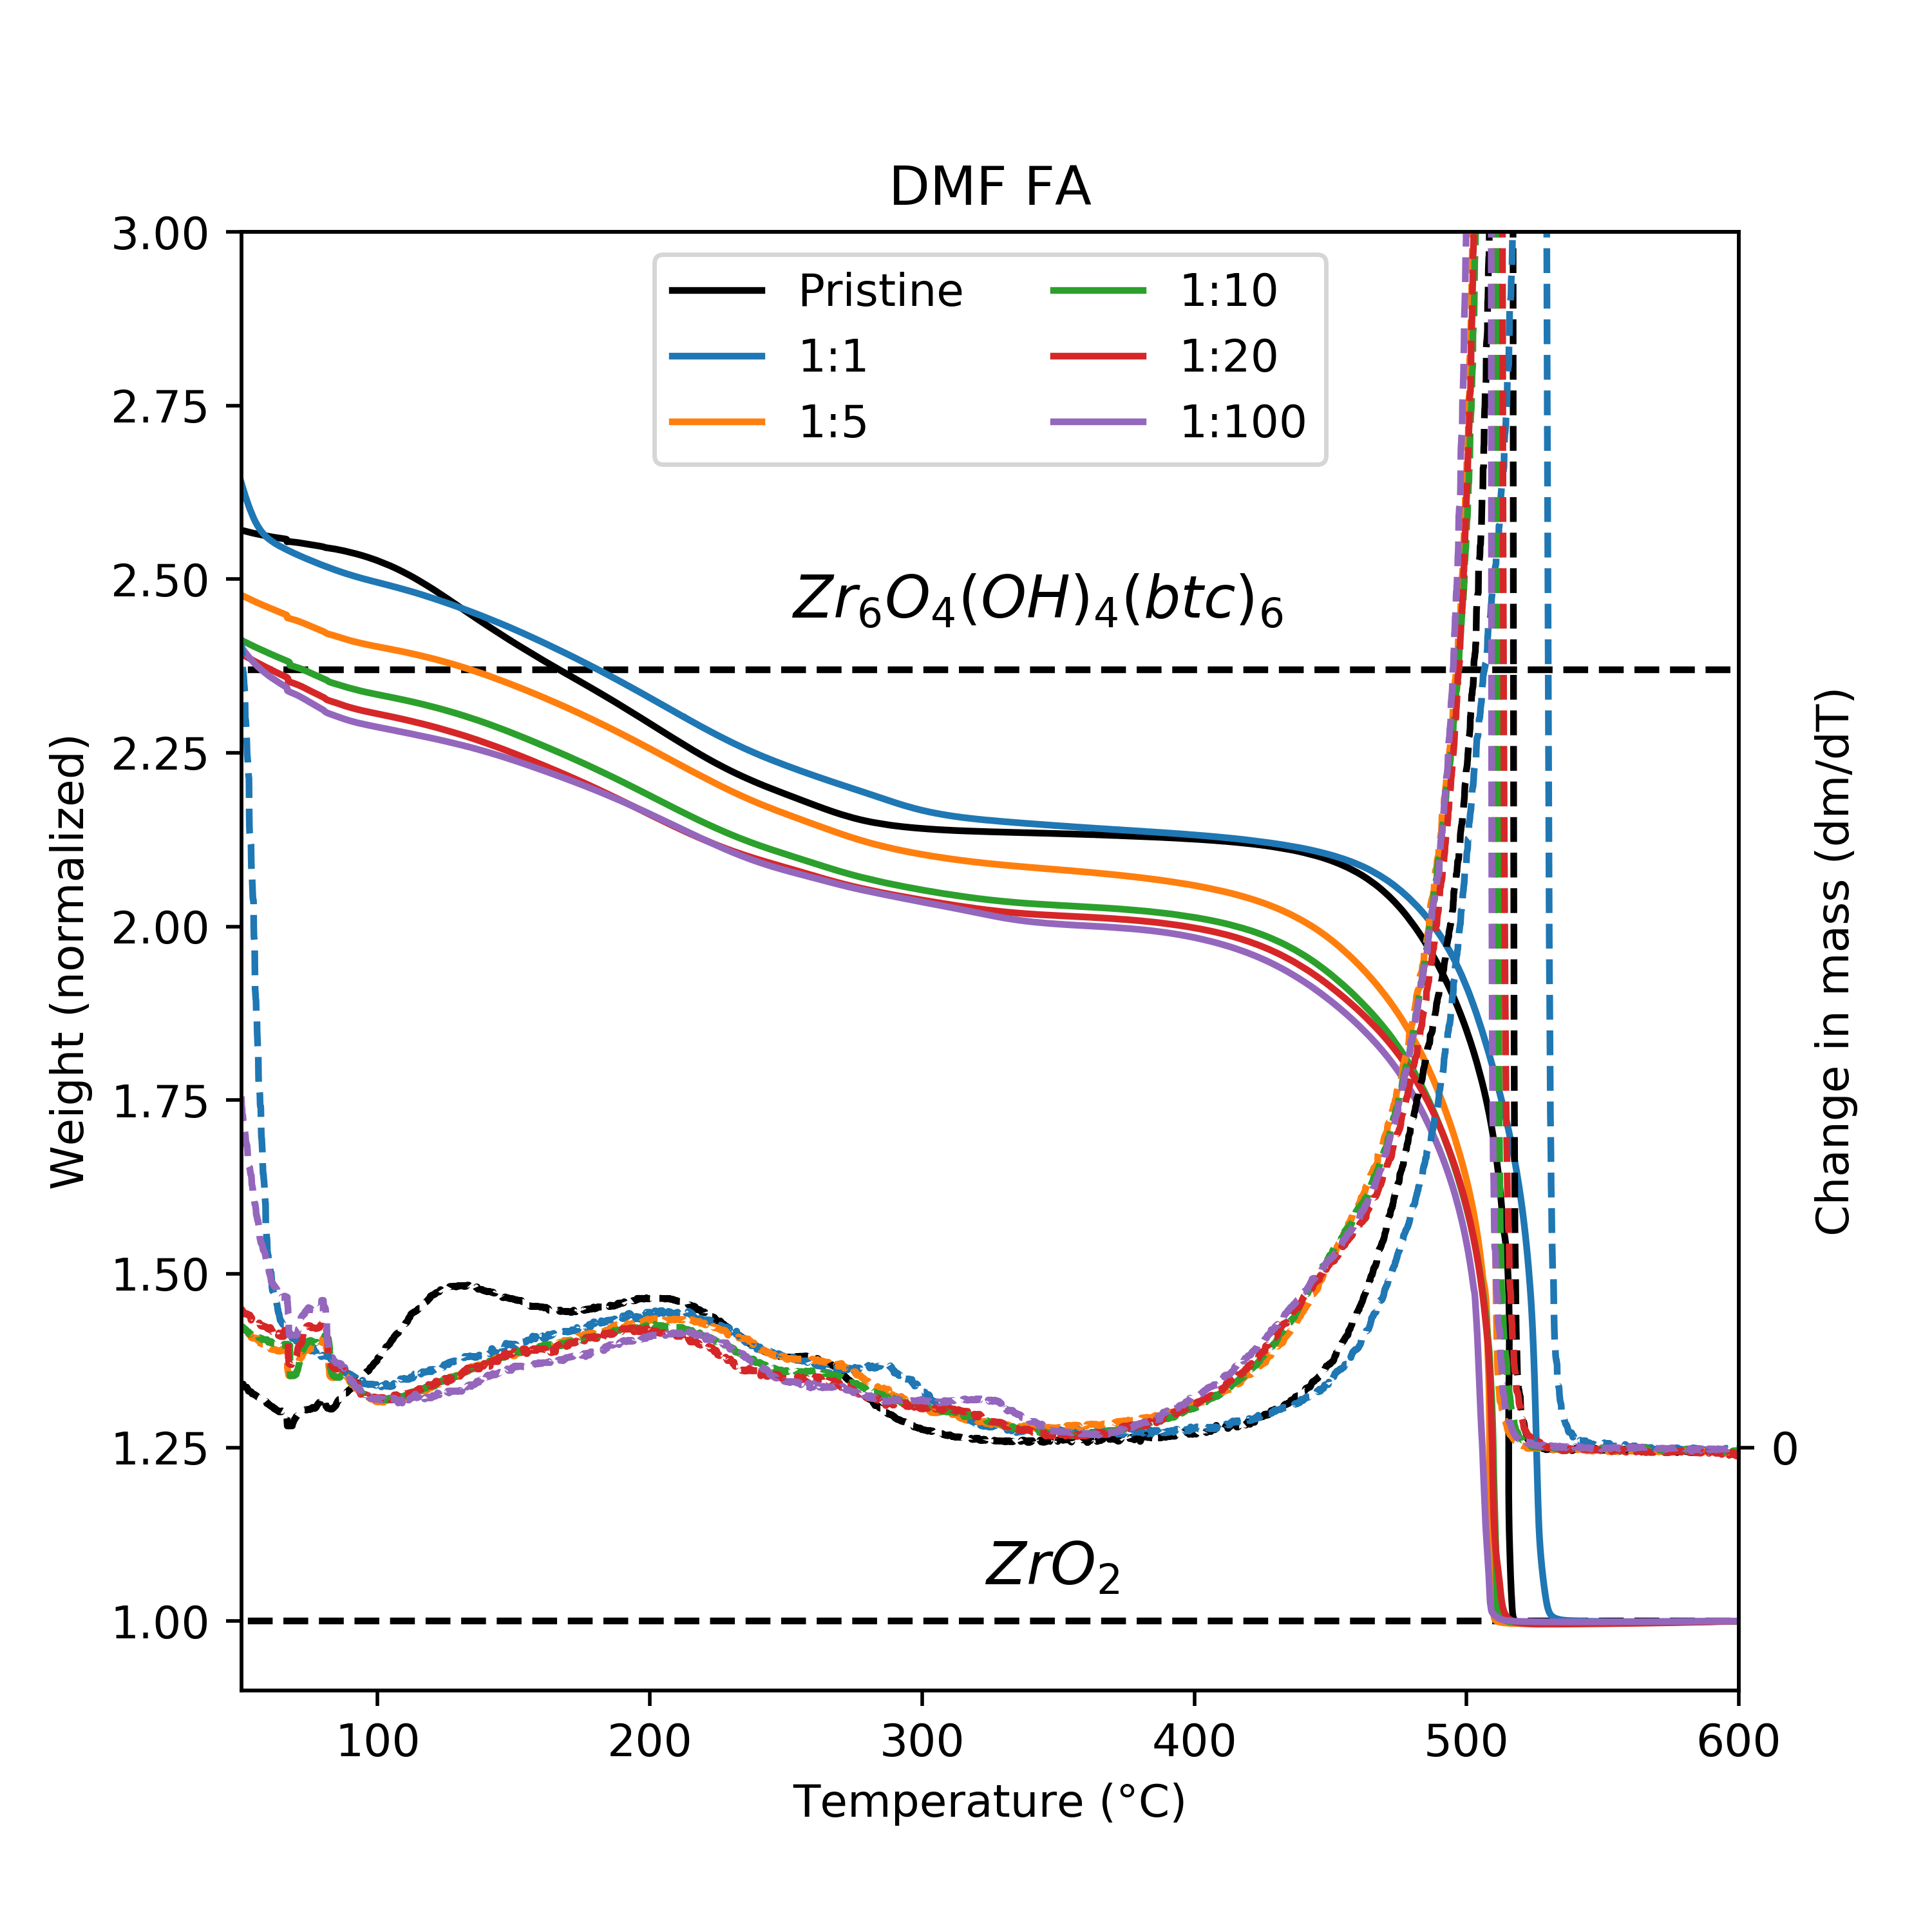
\includegraphics[width=\textwidth]{tga/DMF-FA}%
        \label{appx:def:fgr:tga-dmf-fa}
    \end{subfigure}%
    \begin{subfigure}{0.4\linewidth}
        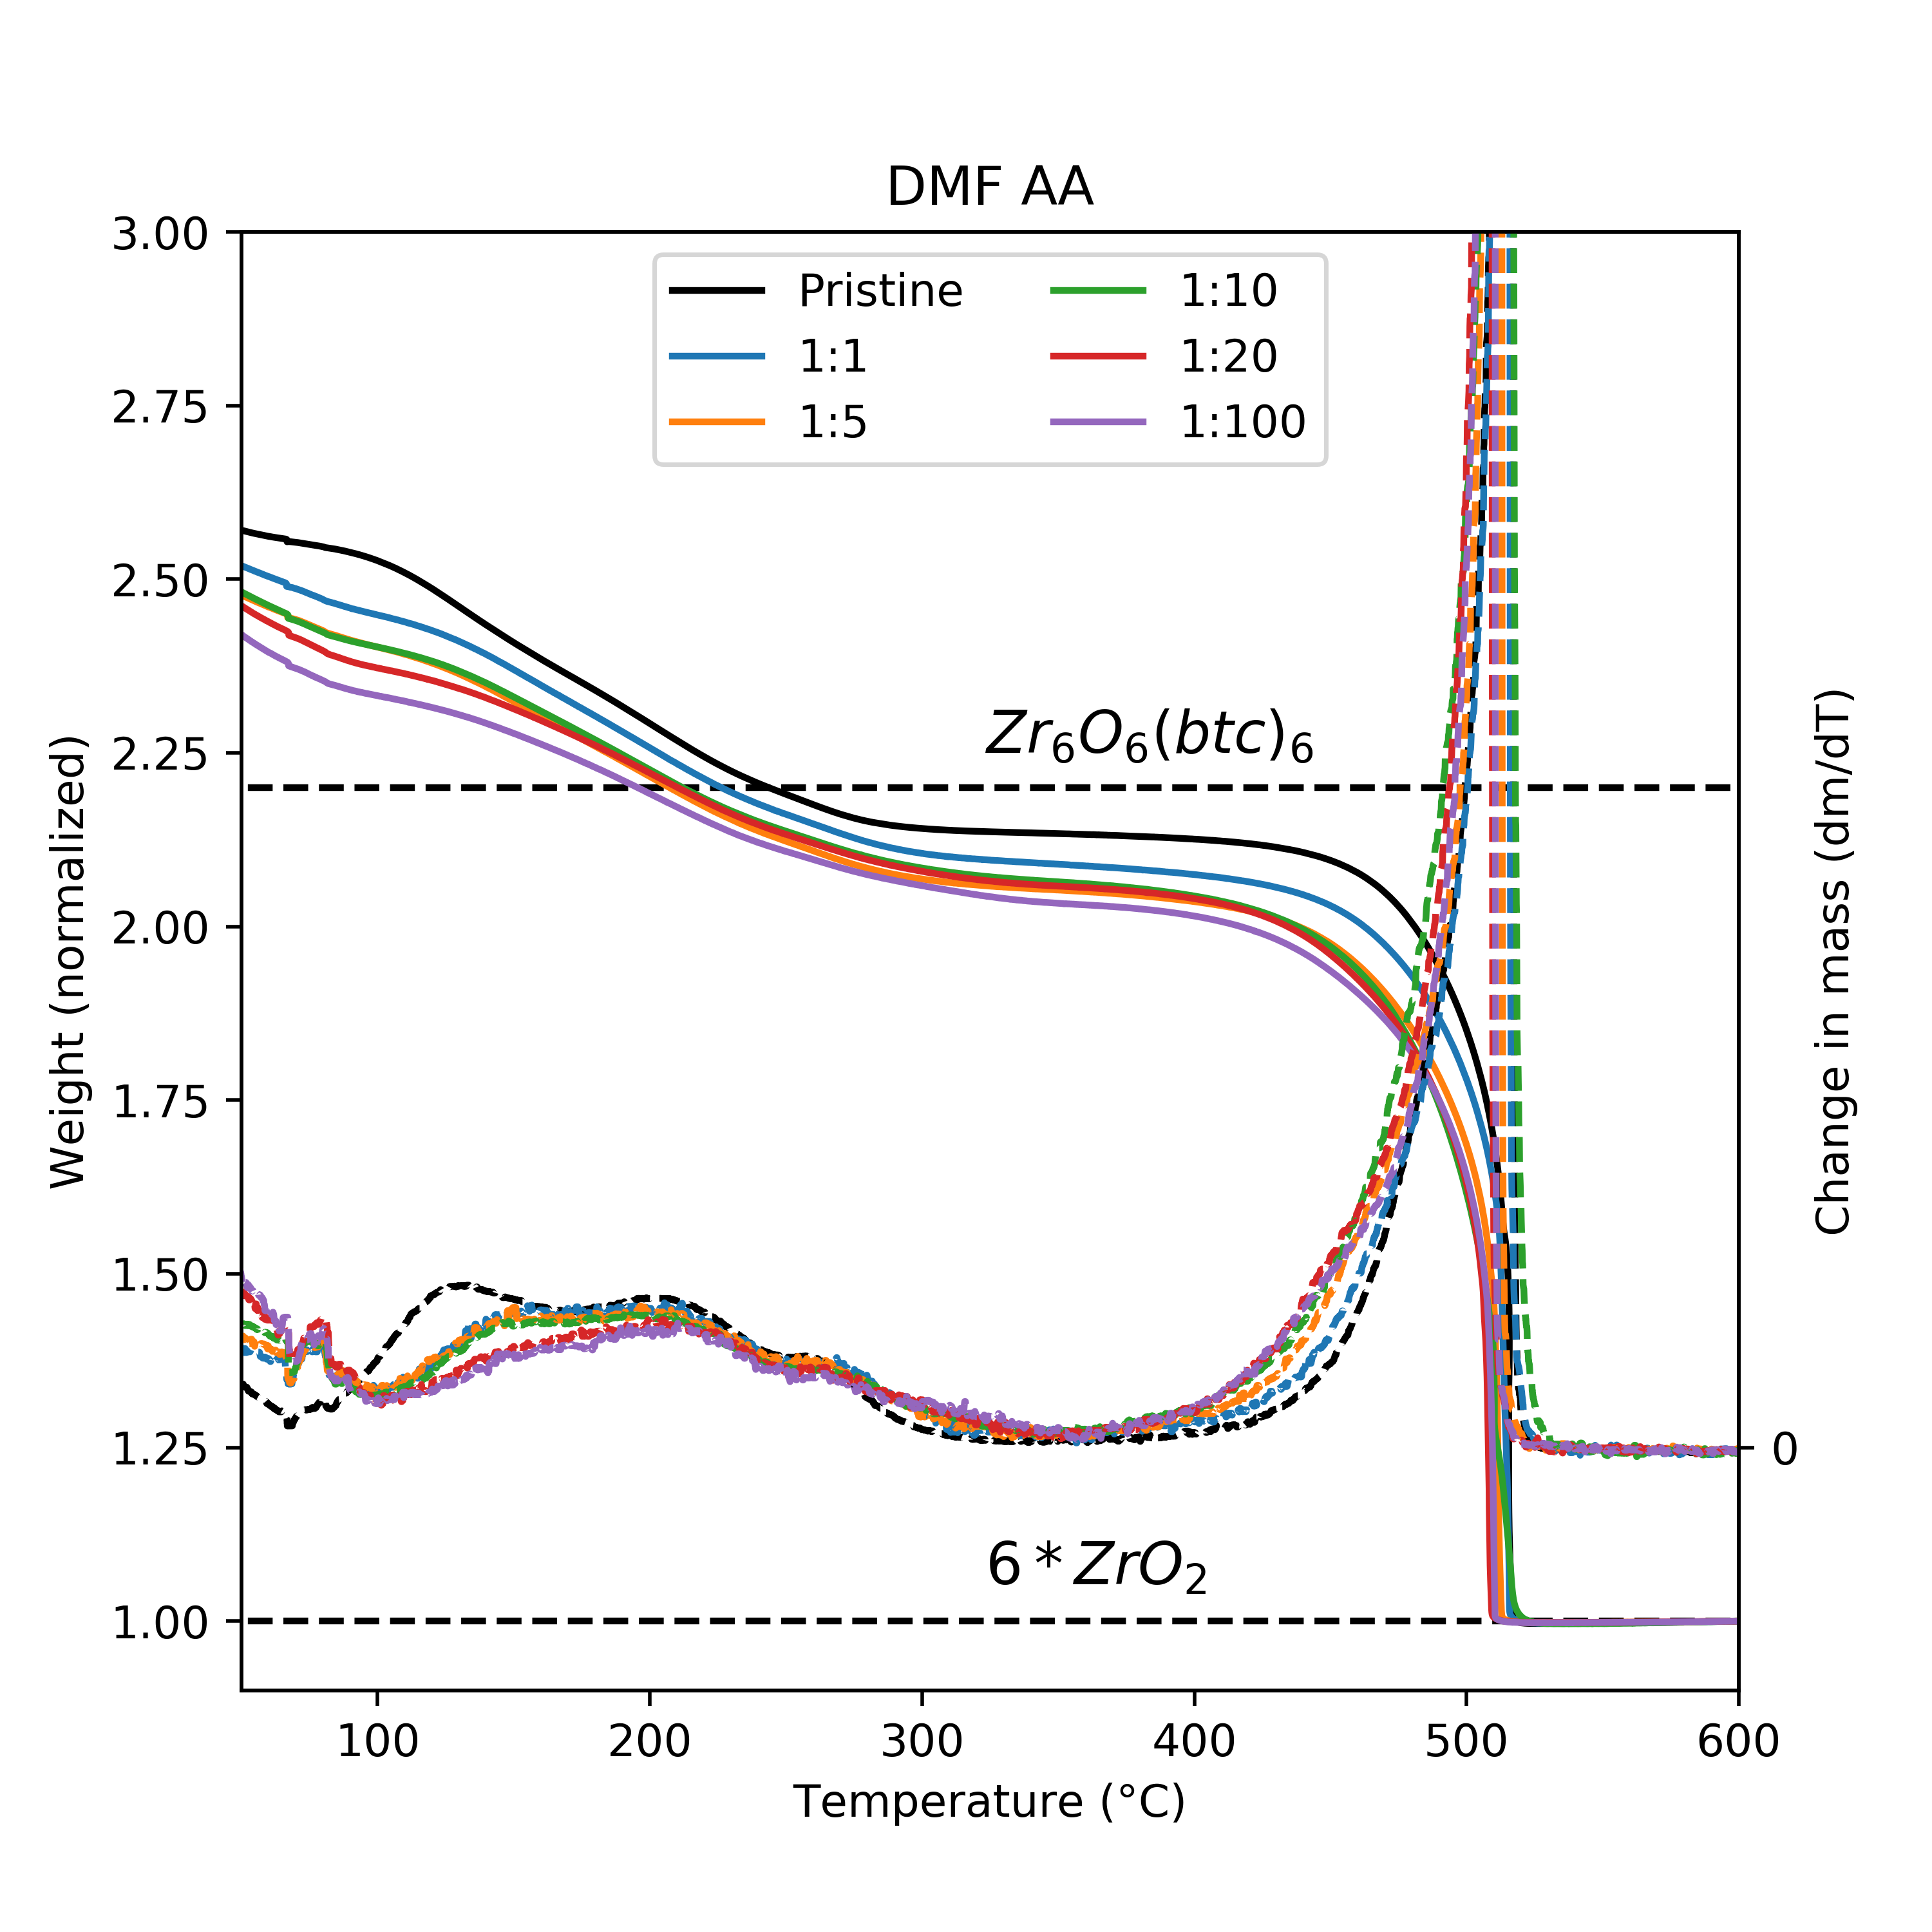
\includegraphics[width=\textwidth]{tga/DMF-AA}%
        \label{appx:def:fgr:tga-dmf-aa}
    \end{subfigure}%

    
    \begin{subfigure}{0.4\linewidth}
        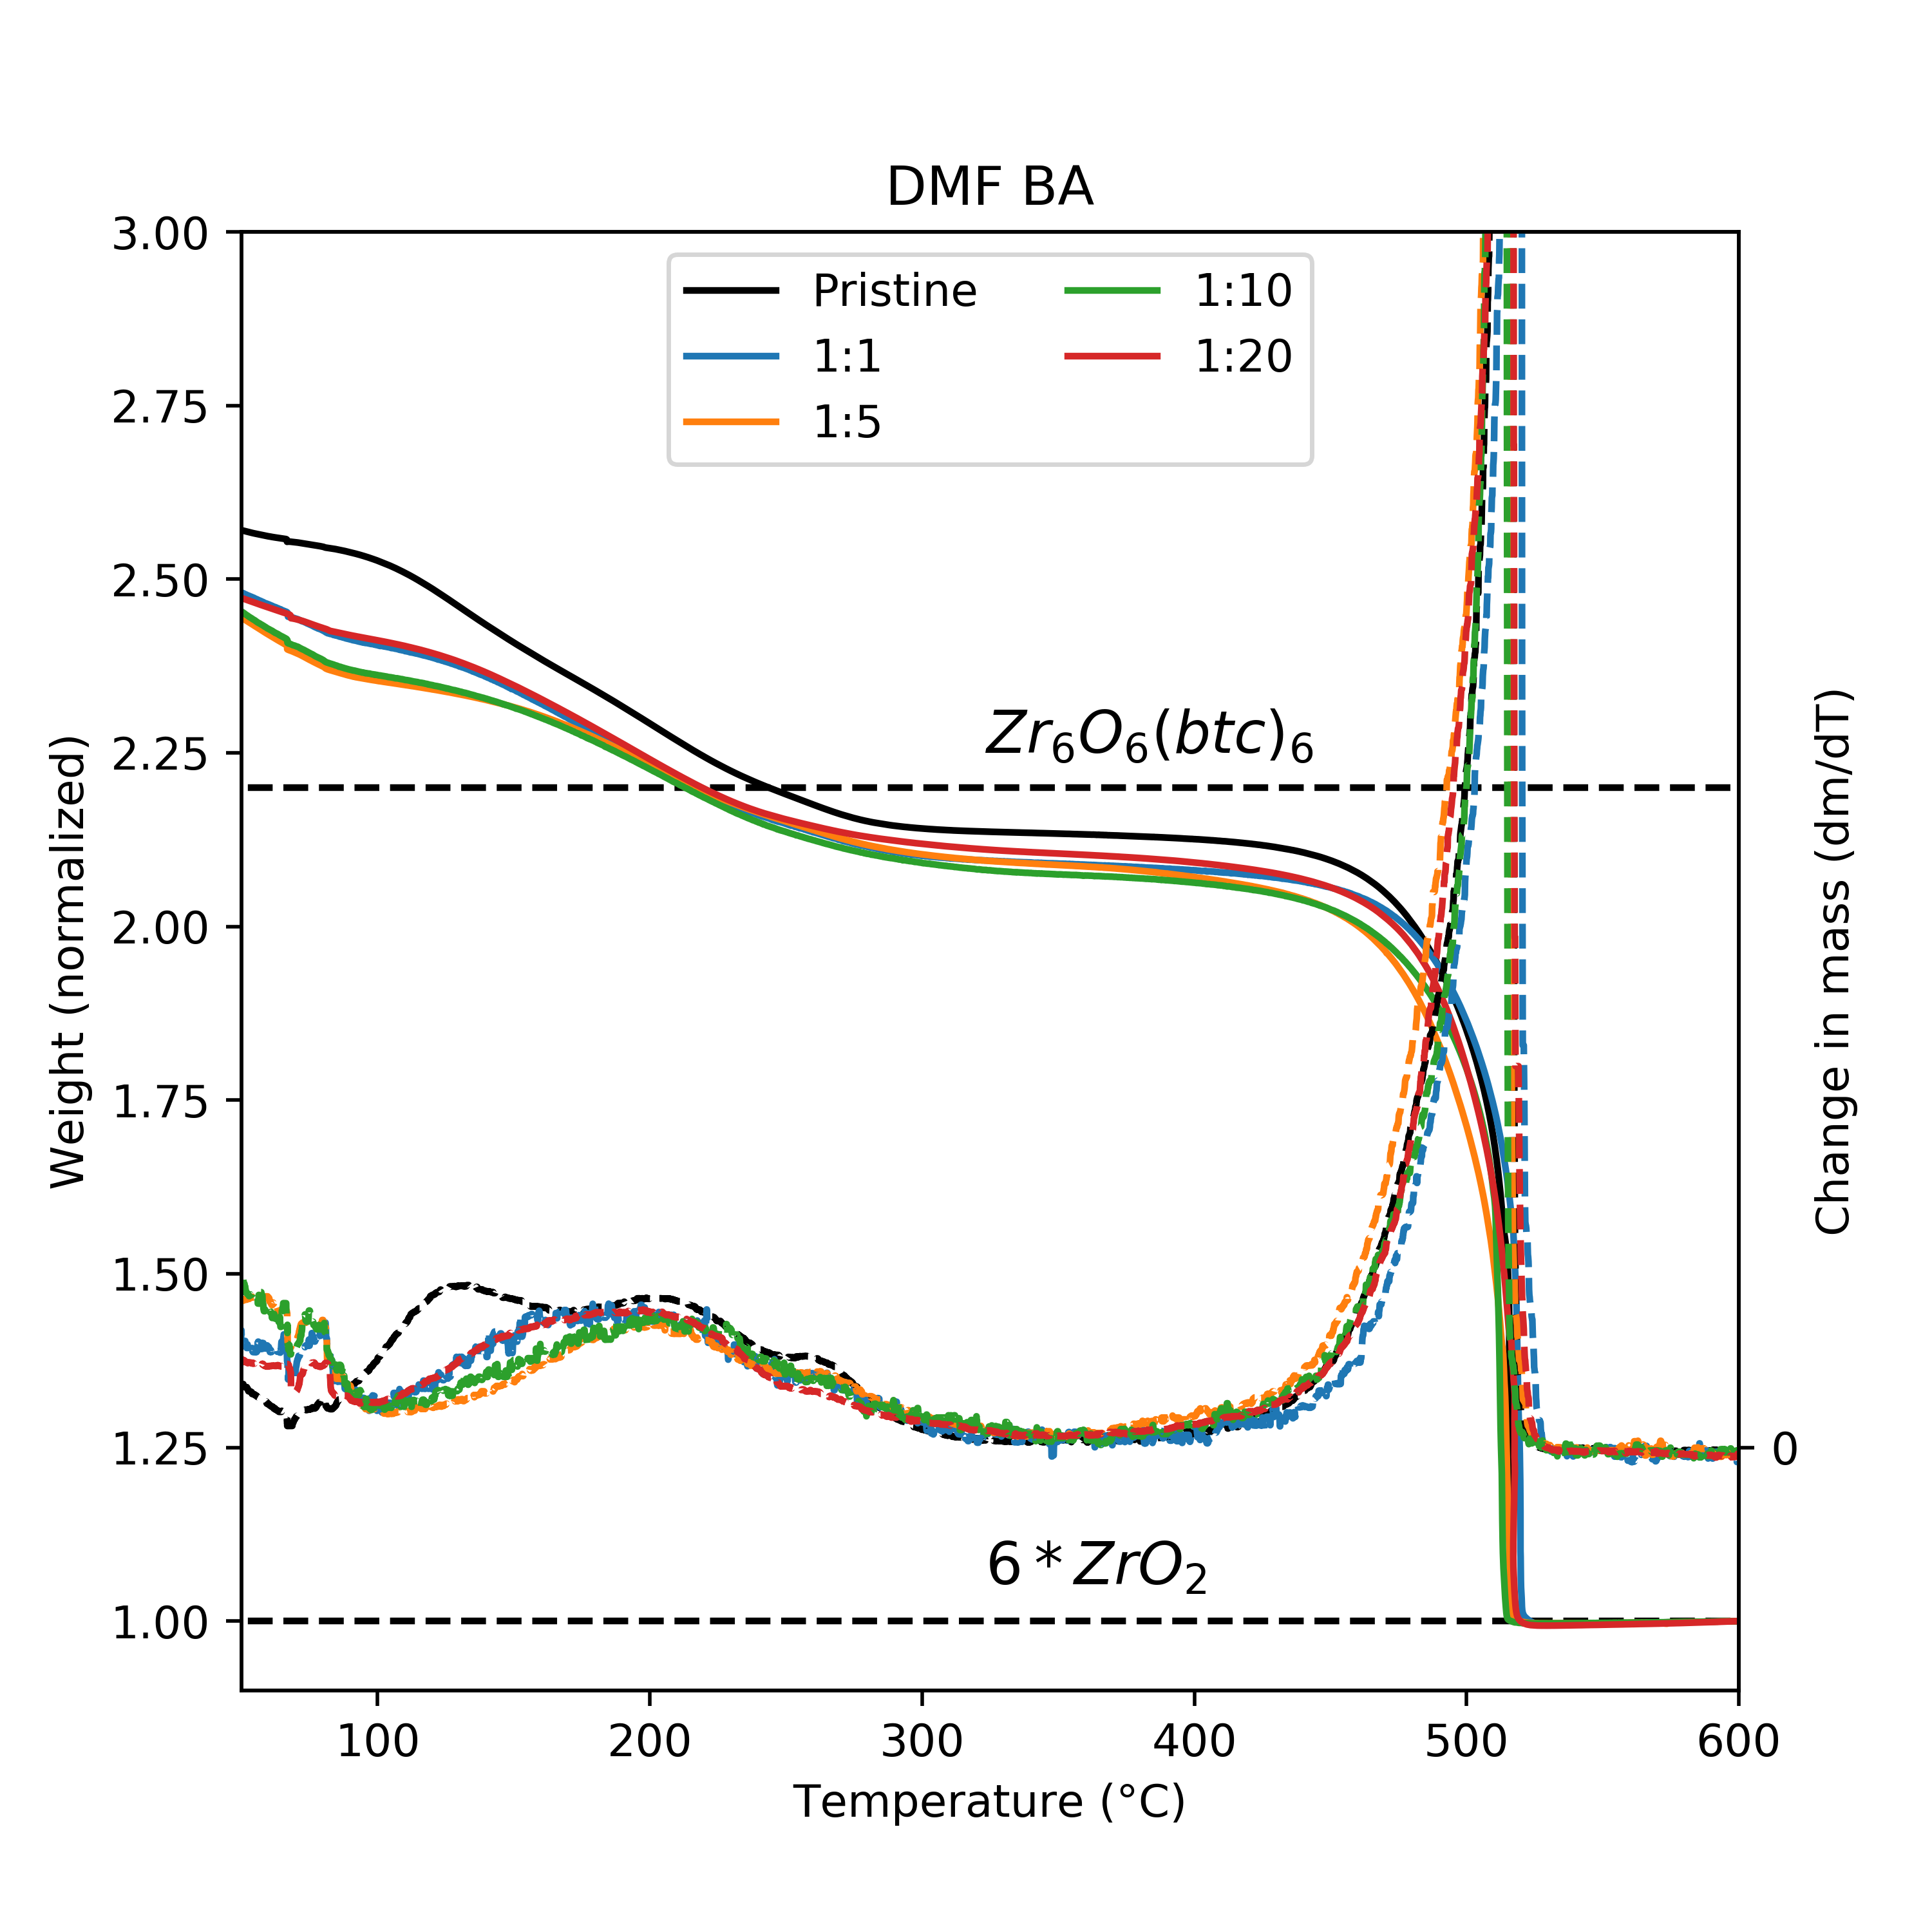
\includegraphics[width=\textwidth]{tga/DMF-BA}%
        \label{appx:def:fgr:tga-dmf-ba}
    \end{subfigure}%

    \caption{TGA curves for samples leached in DMF}%
    \label{appx:def:fgr:tga-dataset}
\end{figure}

\FloatBarrier%
\pagebreak
\subsection{Water leached samples}
\begin{figure}[!h]
    \centering

    \begin{subfigure}{0.4\linewidth}
        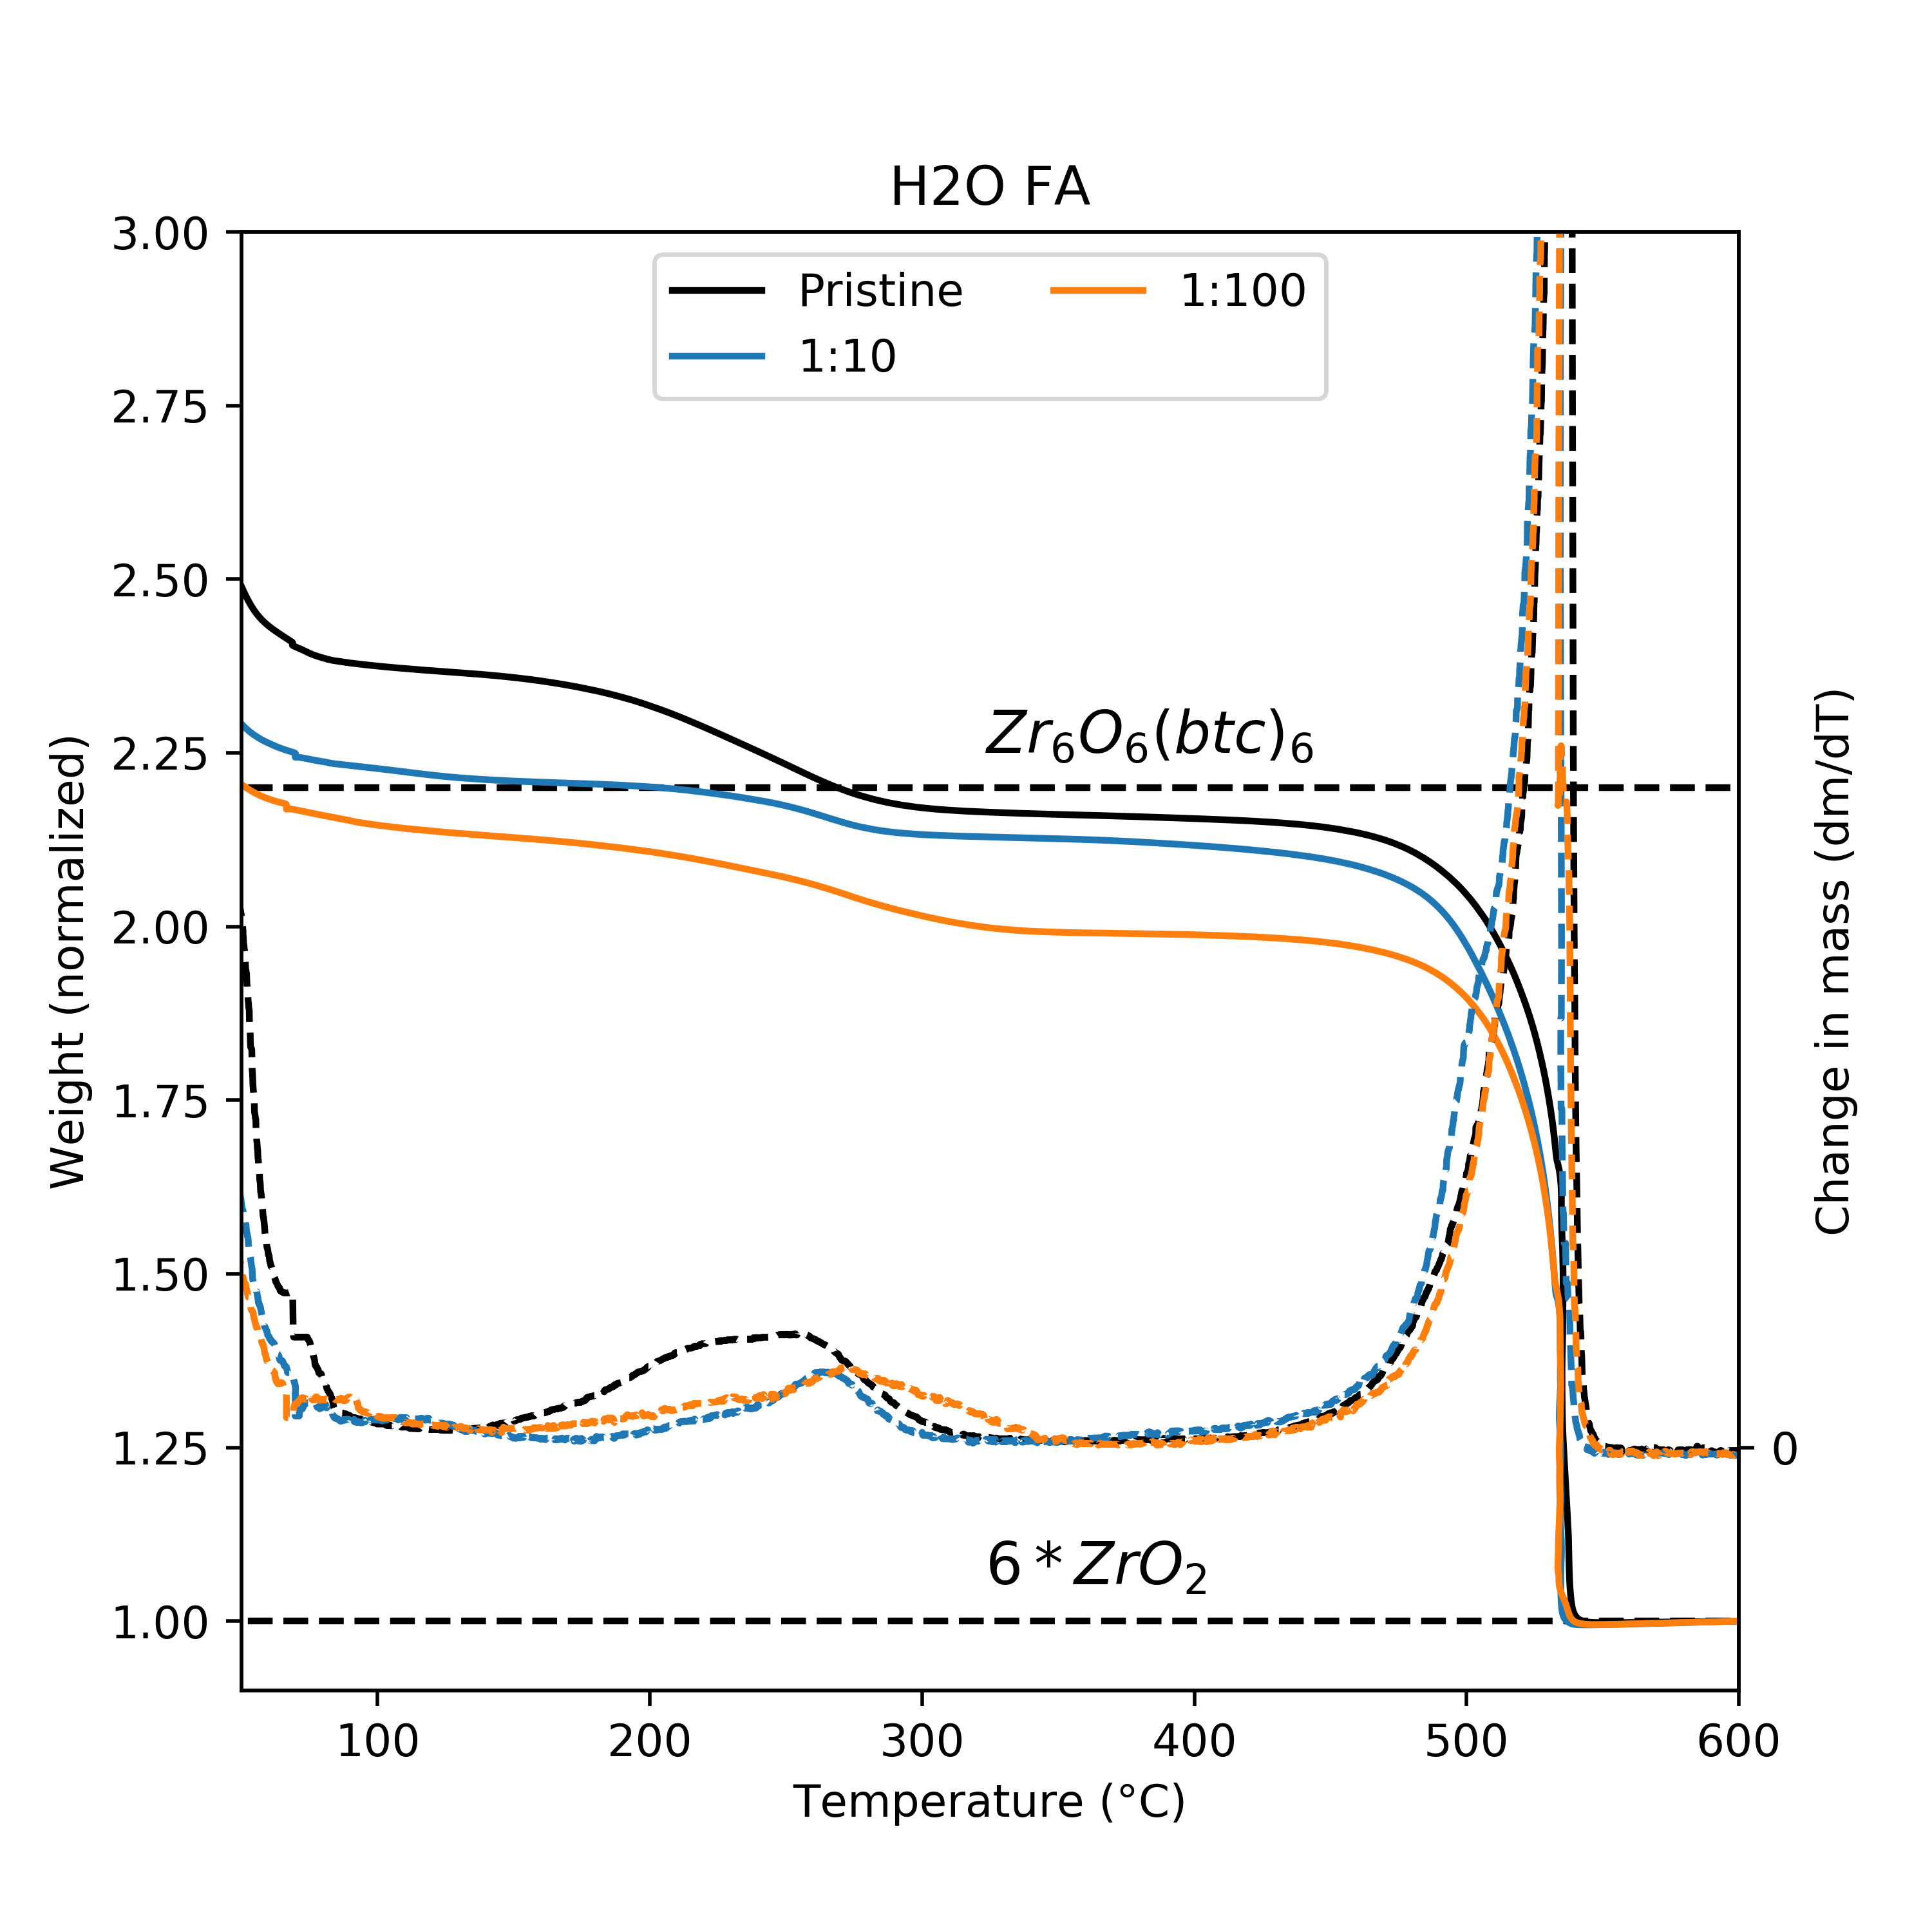
\includegraphics[width=\textwidth]{tga/H2O-FA}%
        \label{appx:def:fgr:tga-h2o-fa}
    \end{subfigure}%
    \begin{subfigure}{0.4\linewidth}
        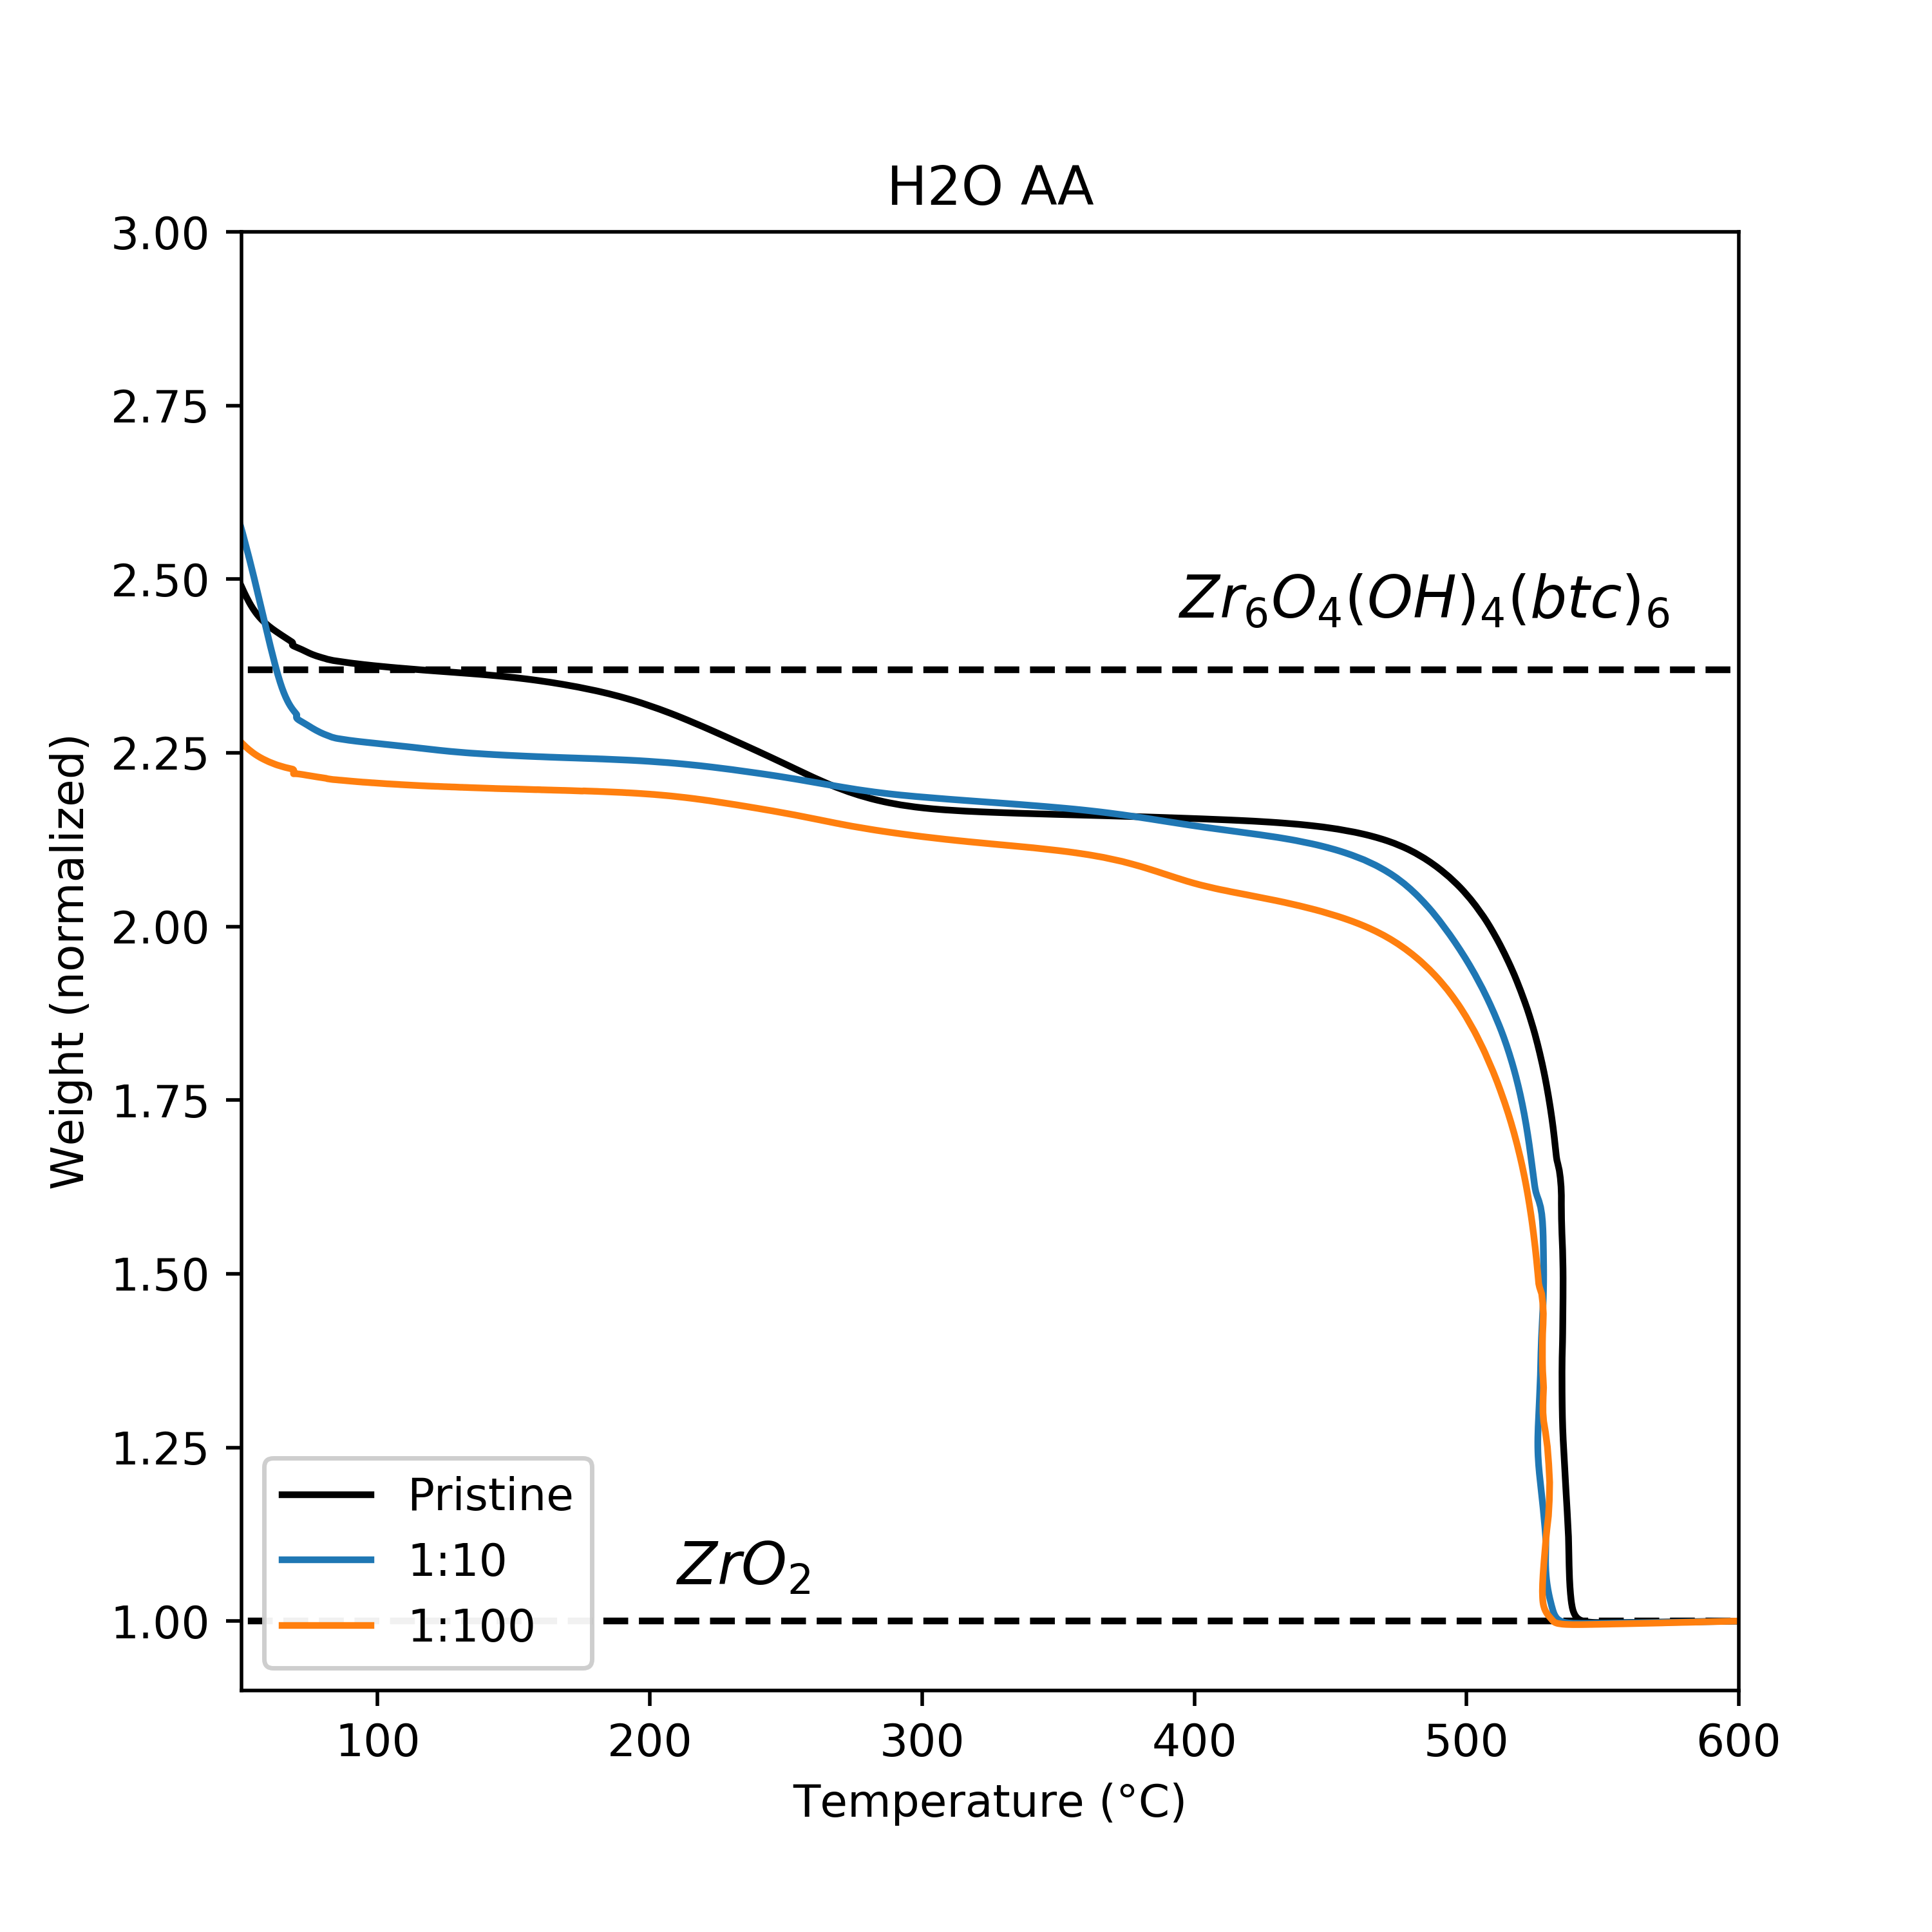
\includegraphics[width=\textwidth]{tga/H2O-AA}%
        \label{appx:def:fgr:tga-h2o-aa}
    \end{subfigure}%

    \begin{subfigure}{0.4\linewidth}
        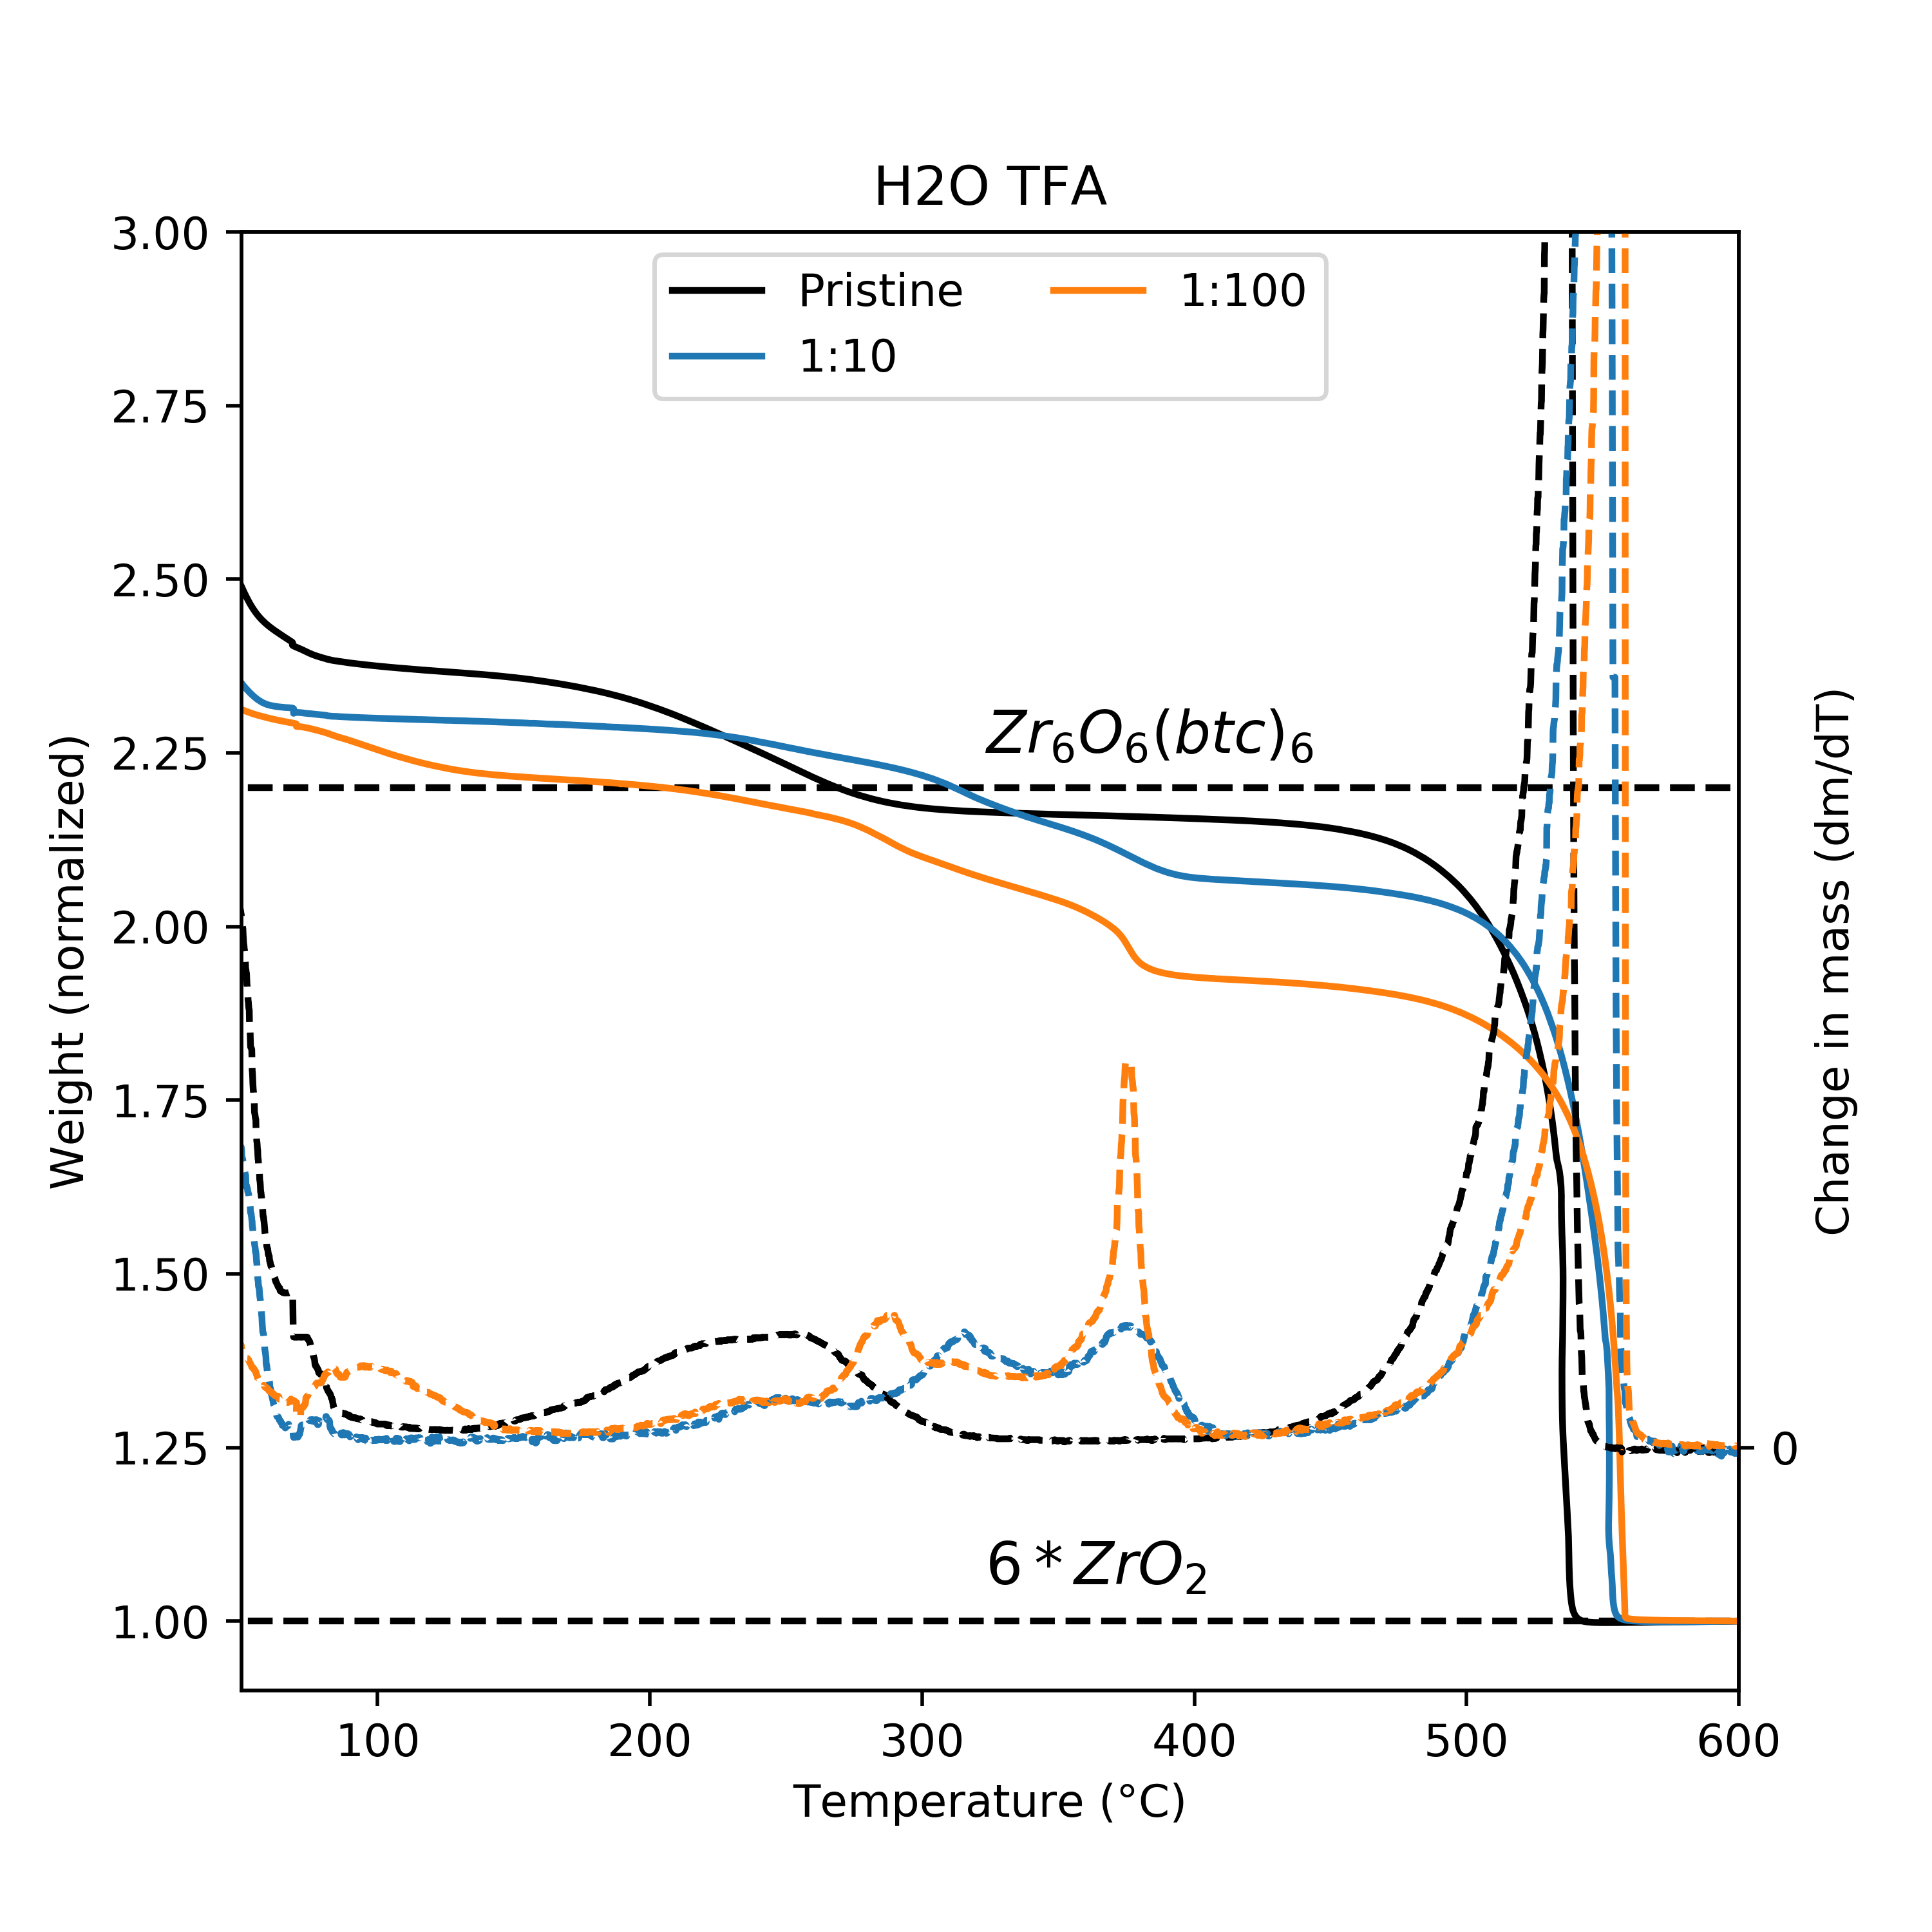
\includegraphics[width=\textwidth]{tga/H2O-TFA}%
        \label{appx:def:fgr:tga-h2o-tfa}
    \end{subfigure}%

    \caption{TGA curves for samples leached in \ce{H2O}}%
\end{figure}

\FloatBarrier%
\pagebreak
\subsection{Methanol leached samples}
\begin{figure}[!h]
    \centering

    \begin{subfigure}{0.4\linewidth}
        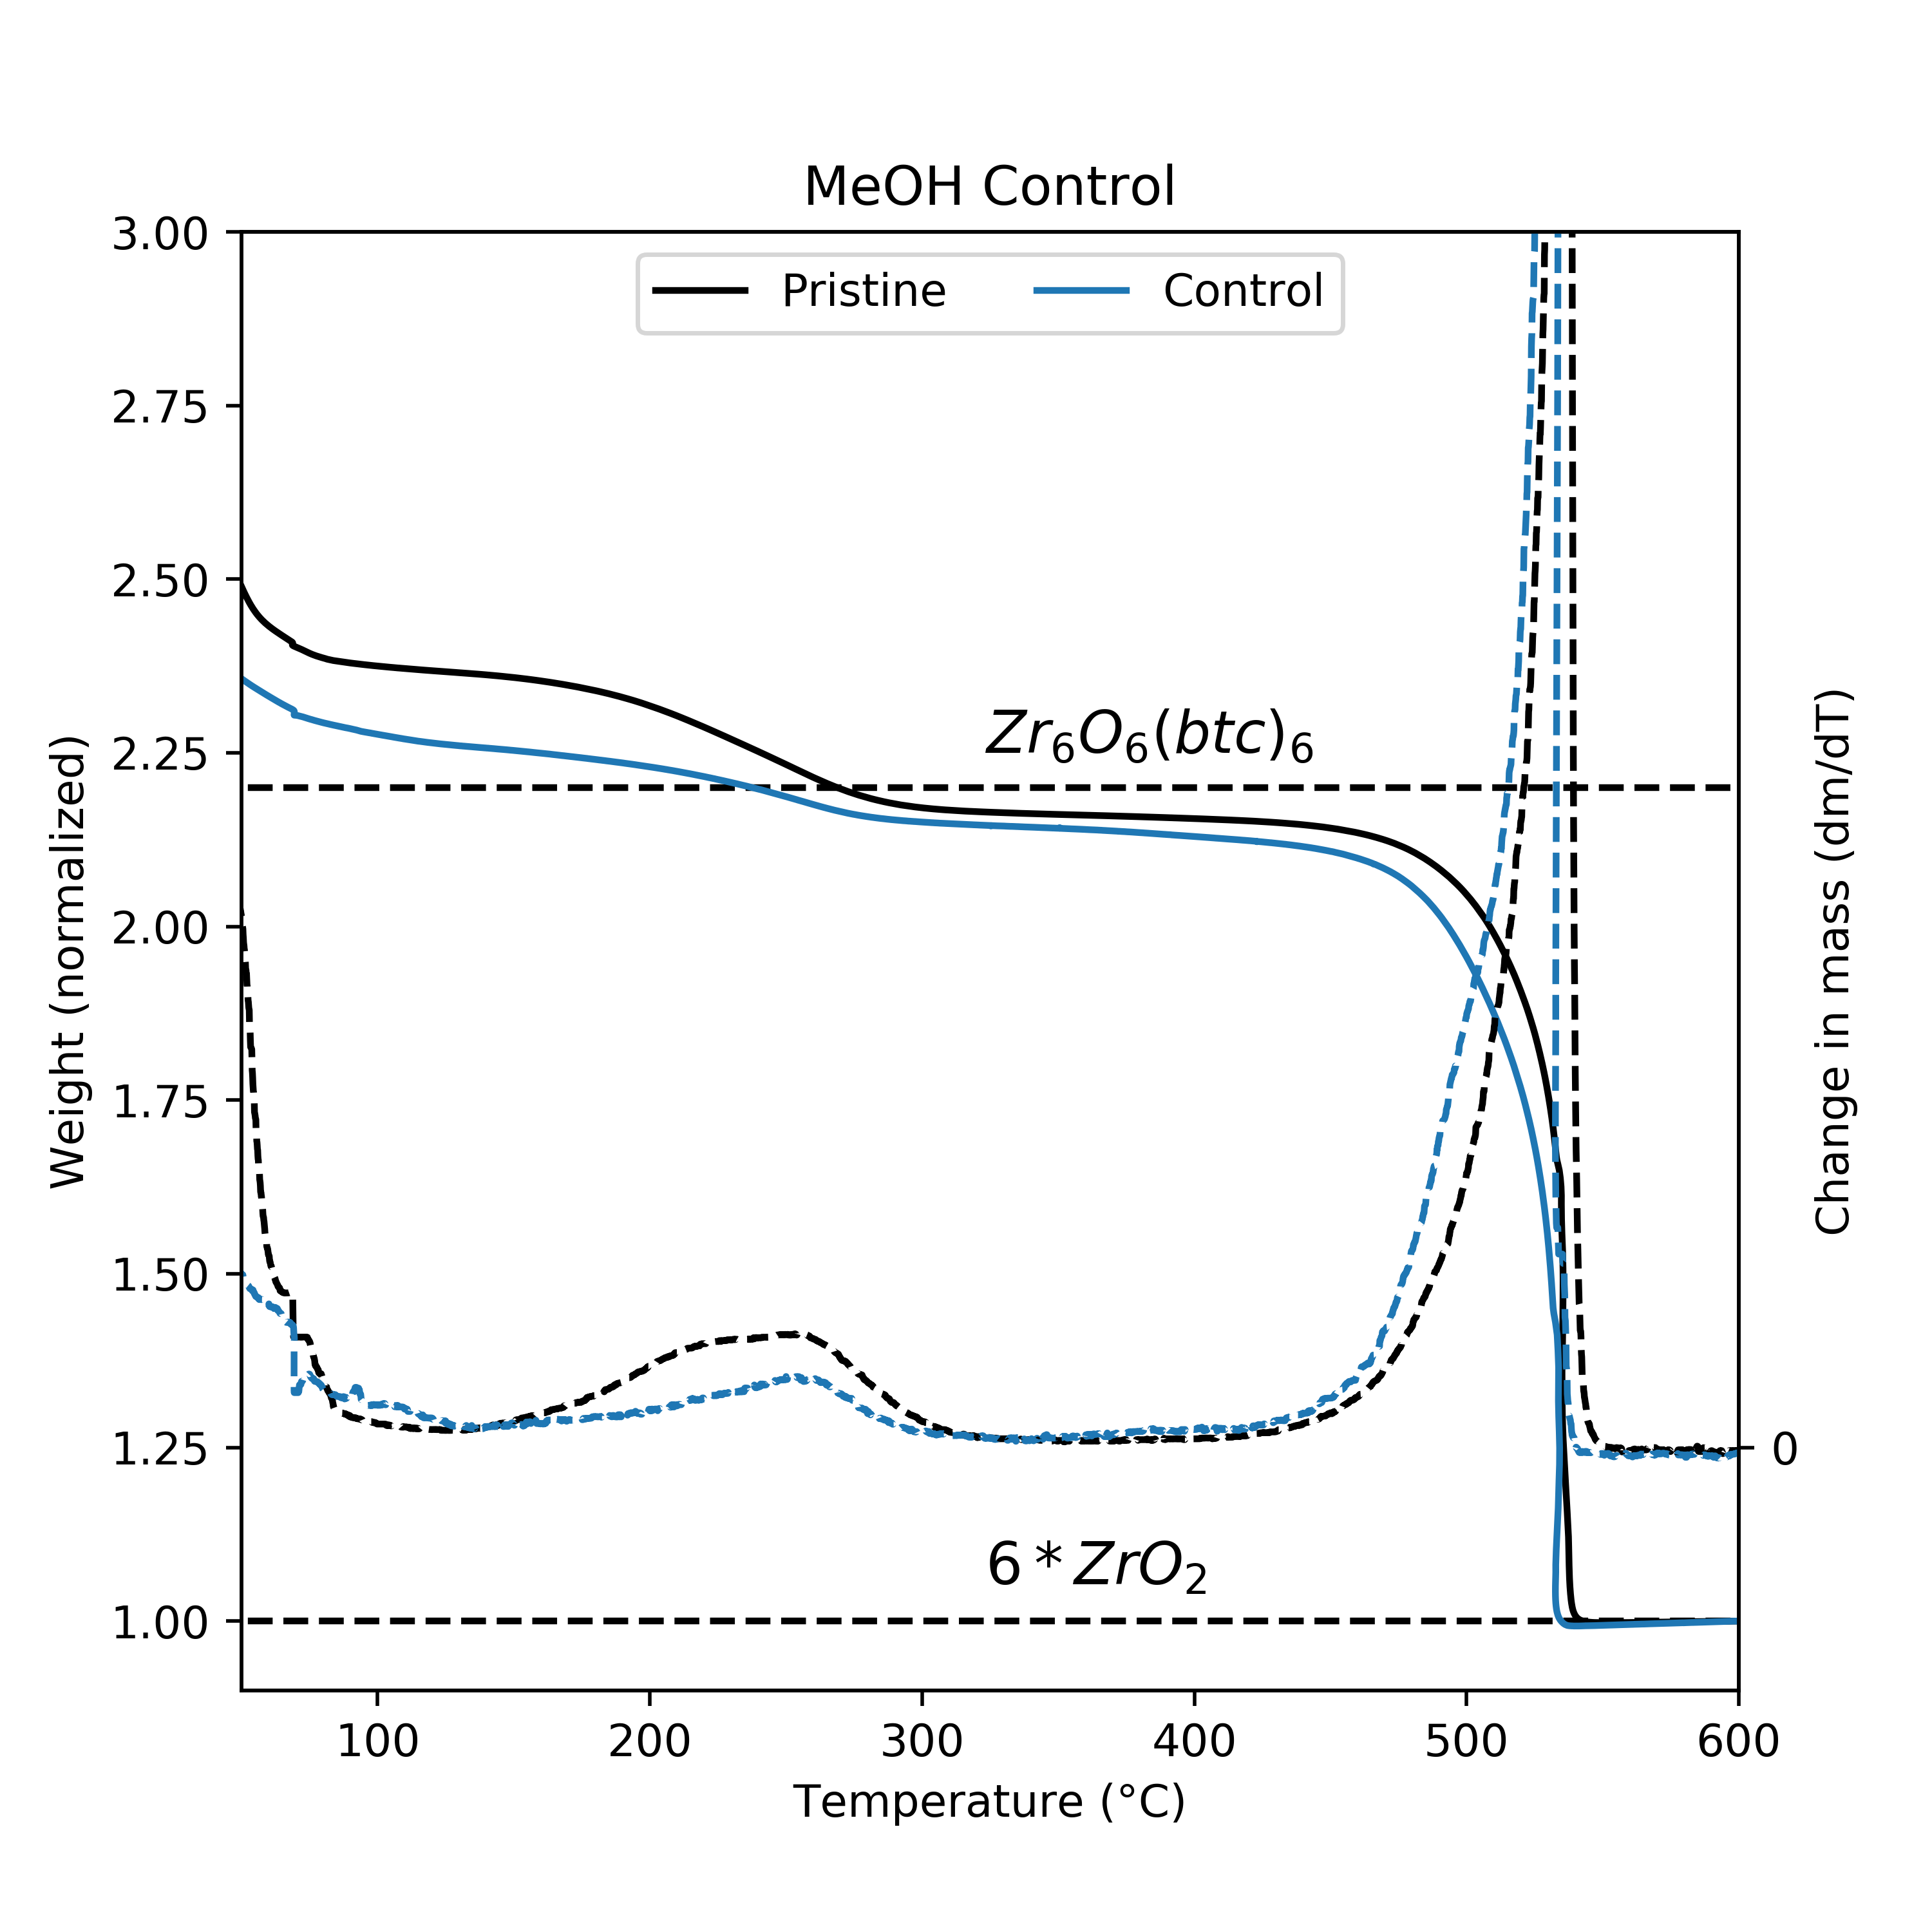
\includegraphics[width=\textwidth]{tga/MeOH-Control}%
        \label{appx:def:fgr:tga-meoh-cont}
    \end{subfigure}%

    \begin{subfigure}{0.4\linewidth}
        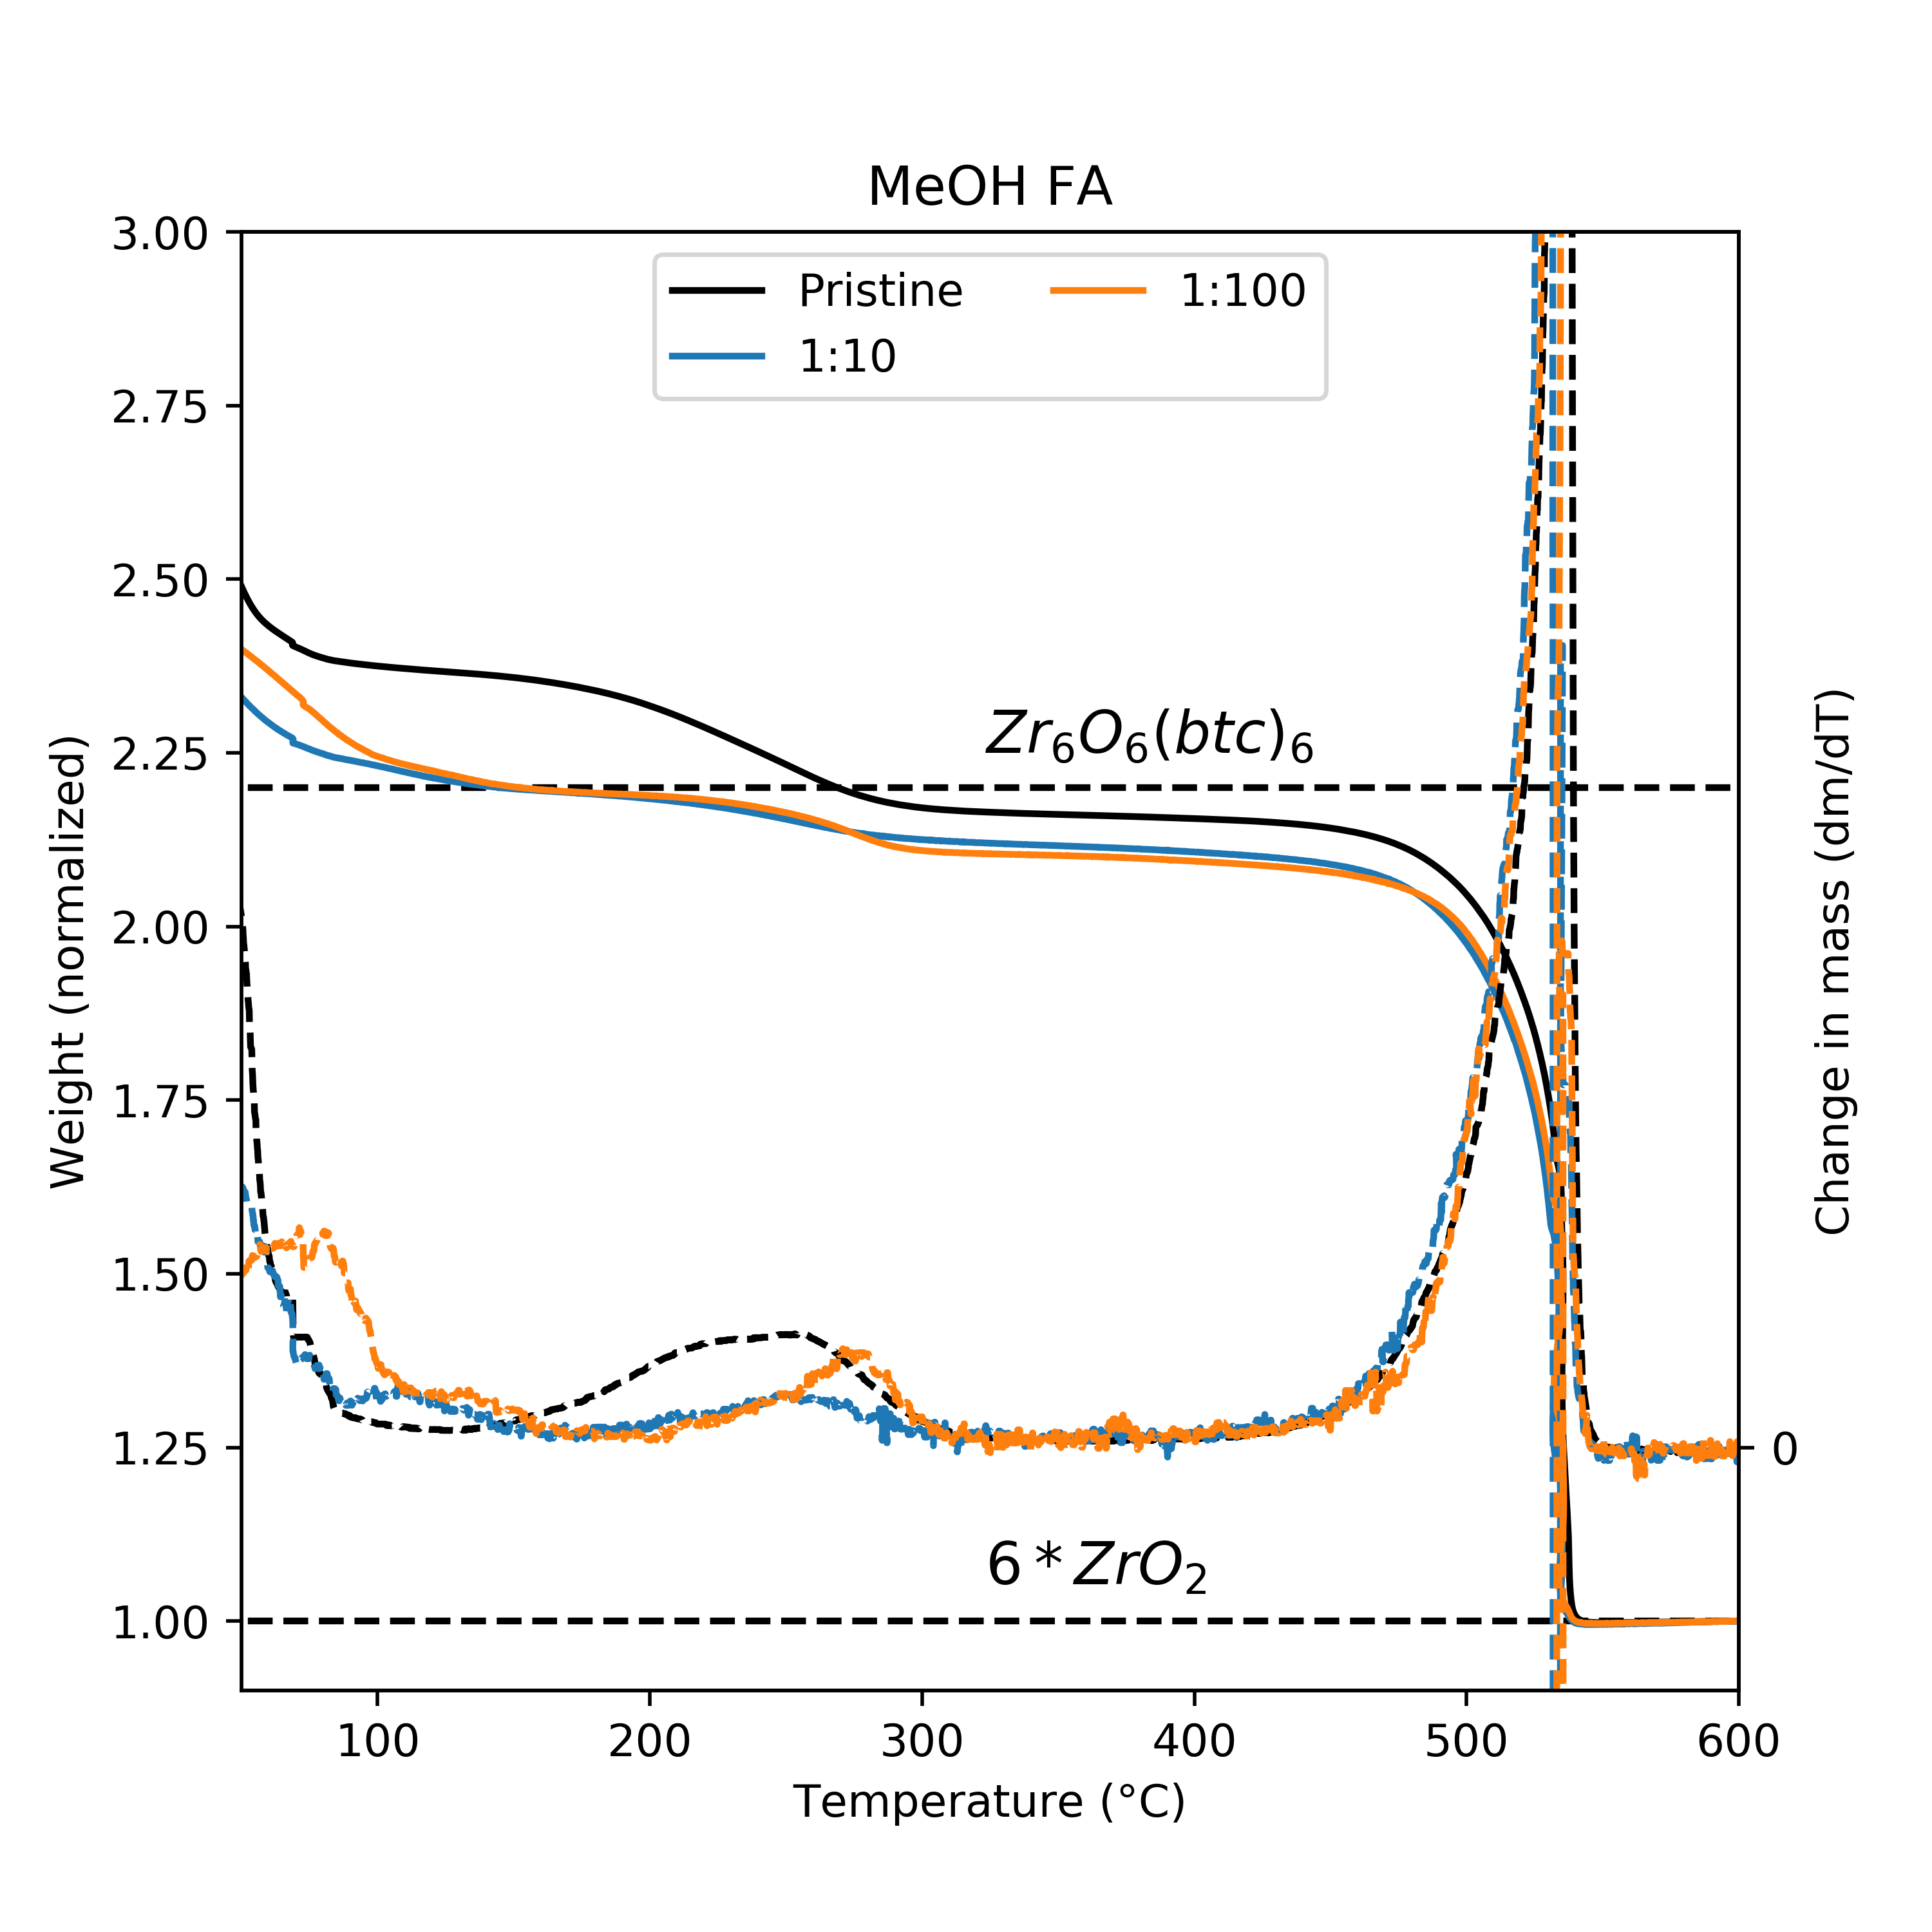
\includegraphics[width=\textwidth]{tga/MeOH-FA}%
        \label{appx:def:fgr:tga-meoh-fa}
    \end{subfigure}%
    \begin{subfigure}{0.4\linewidth}
        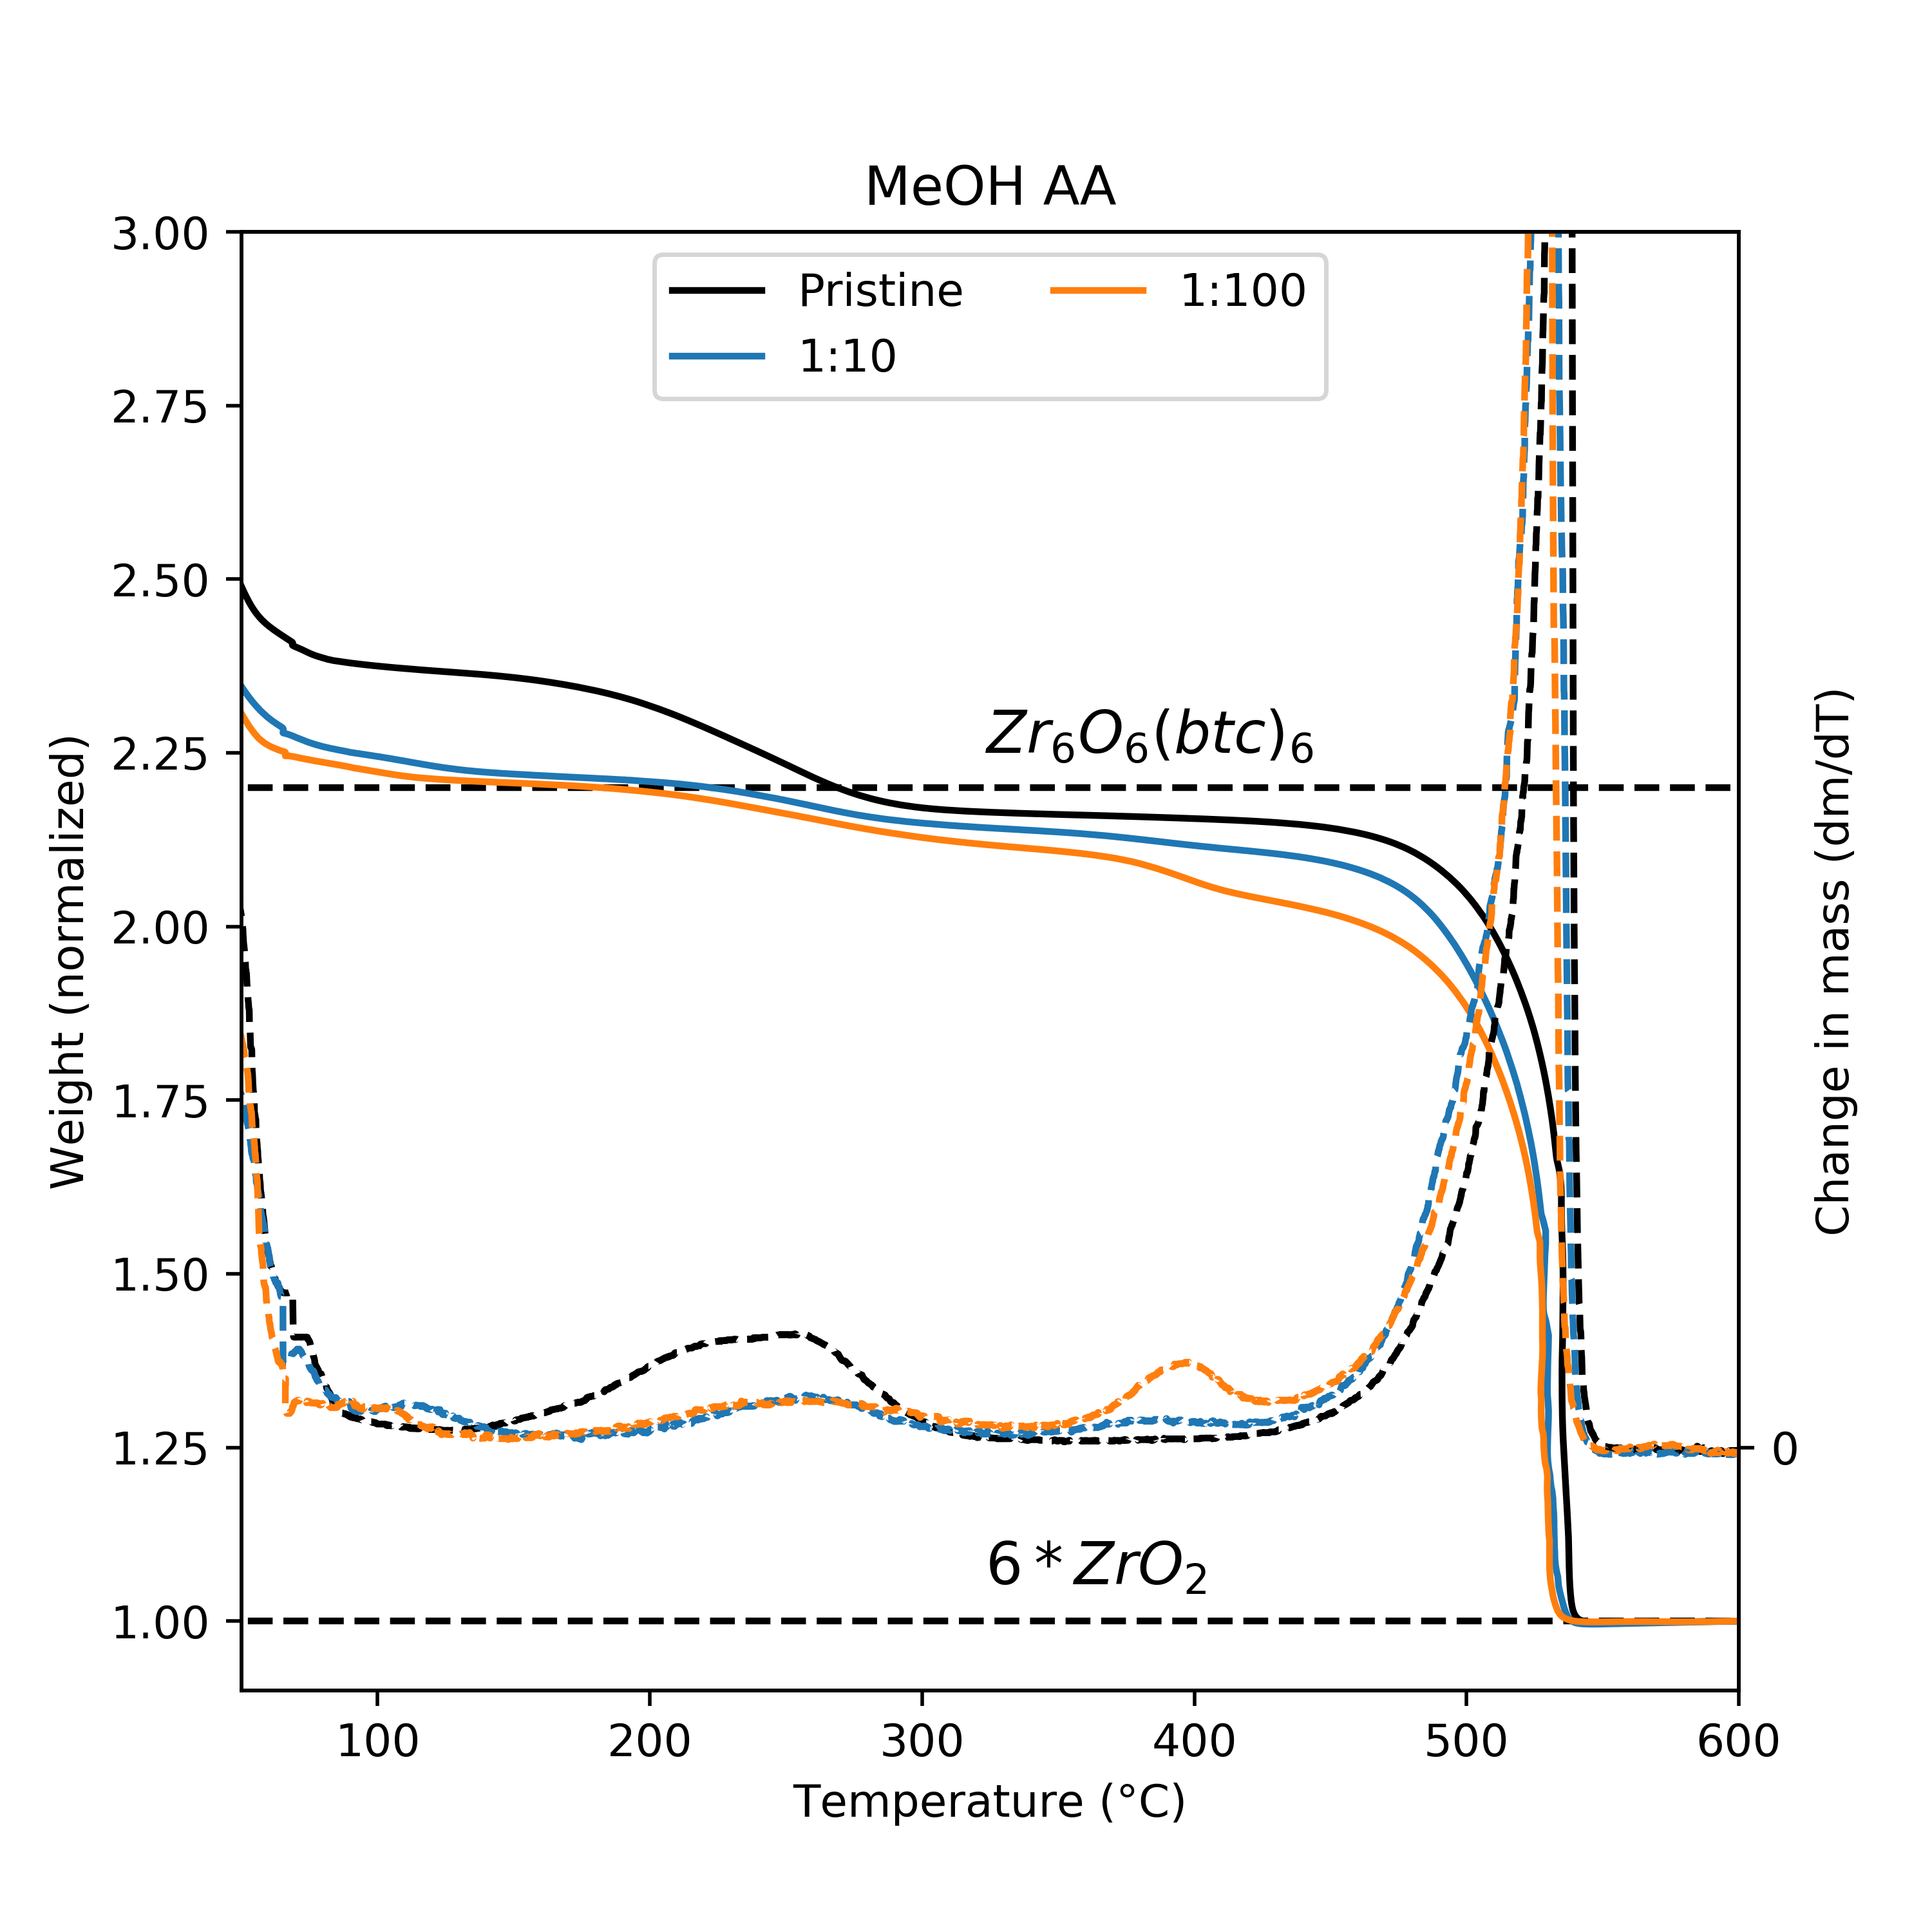
\includegraphics[width=\textwidth]{tga/MeOH-AA}%
        \label{appx:def:fgr:tga-meoh-aa}
    \end{subfigure}%
    
    \begin{subfigure}{0.4\linewidth}
        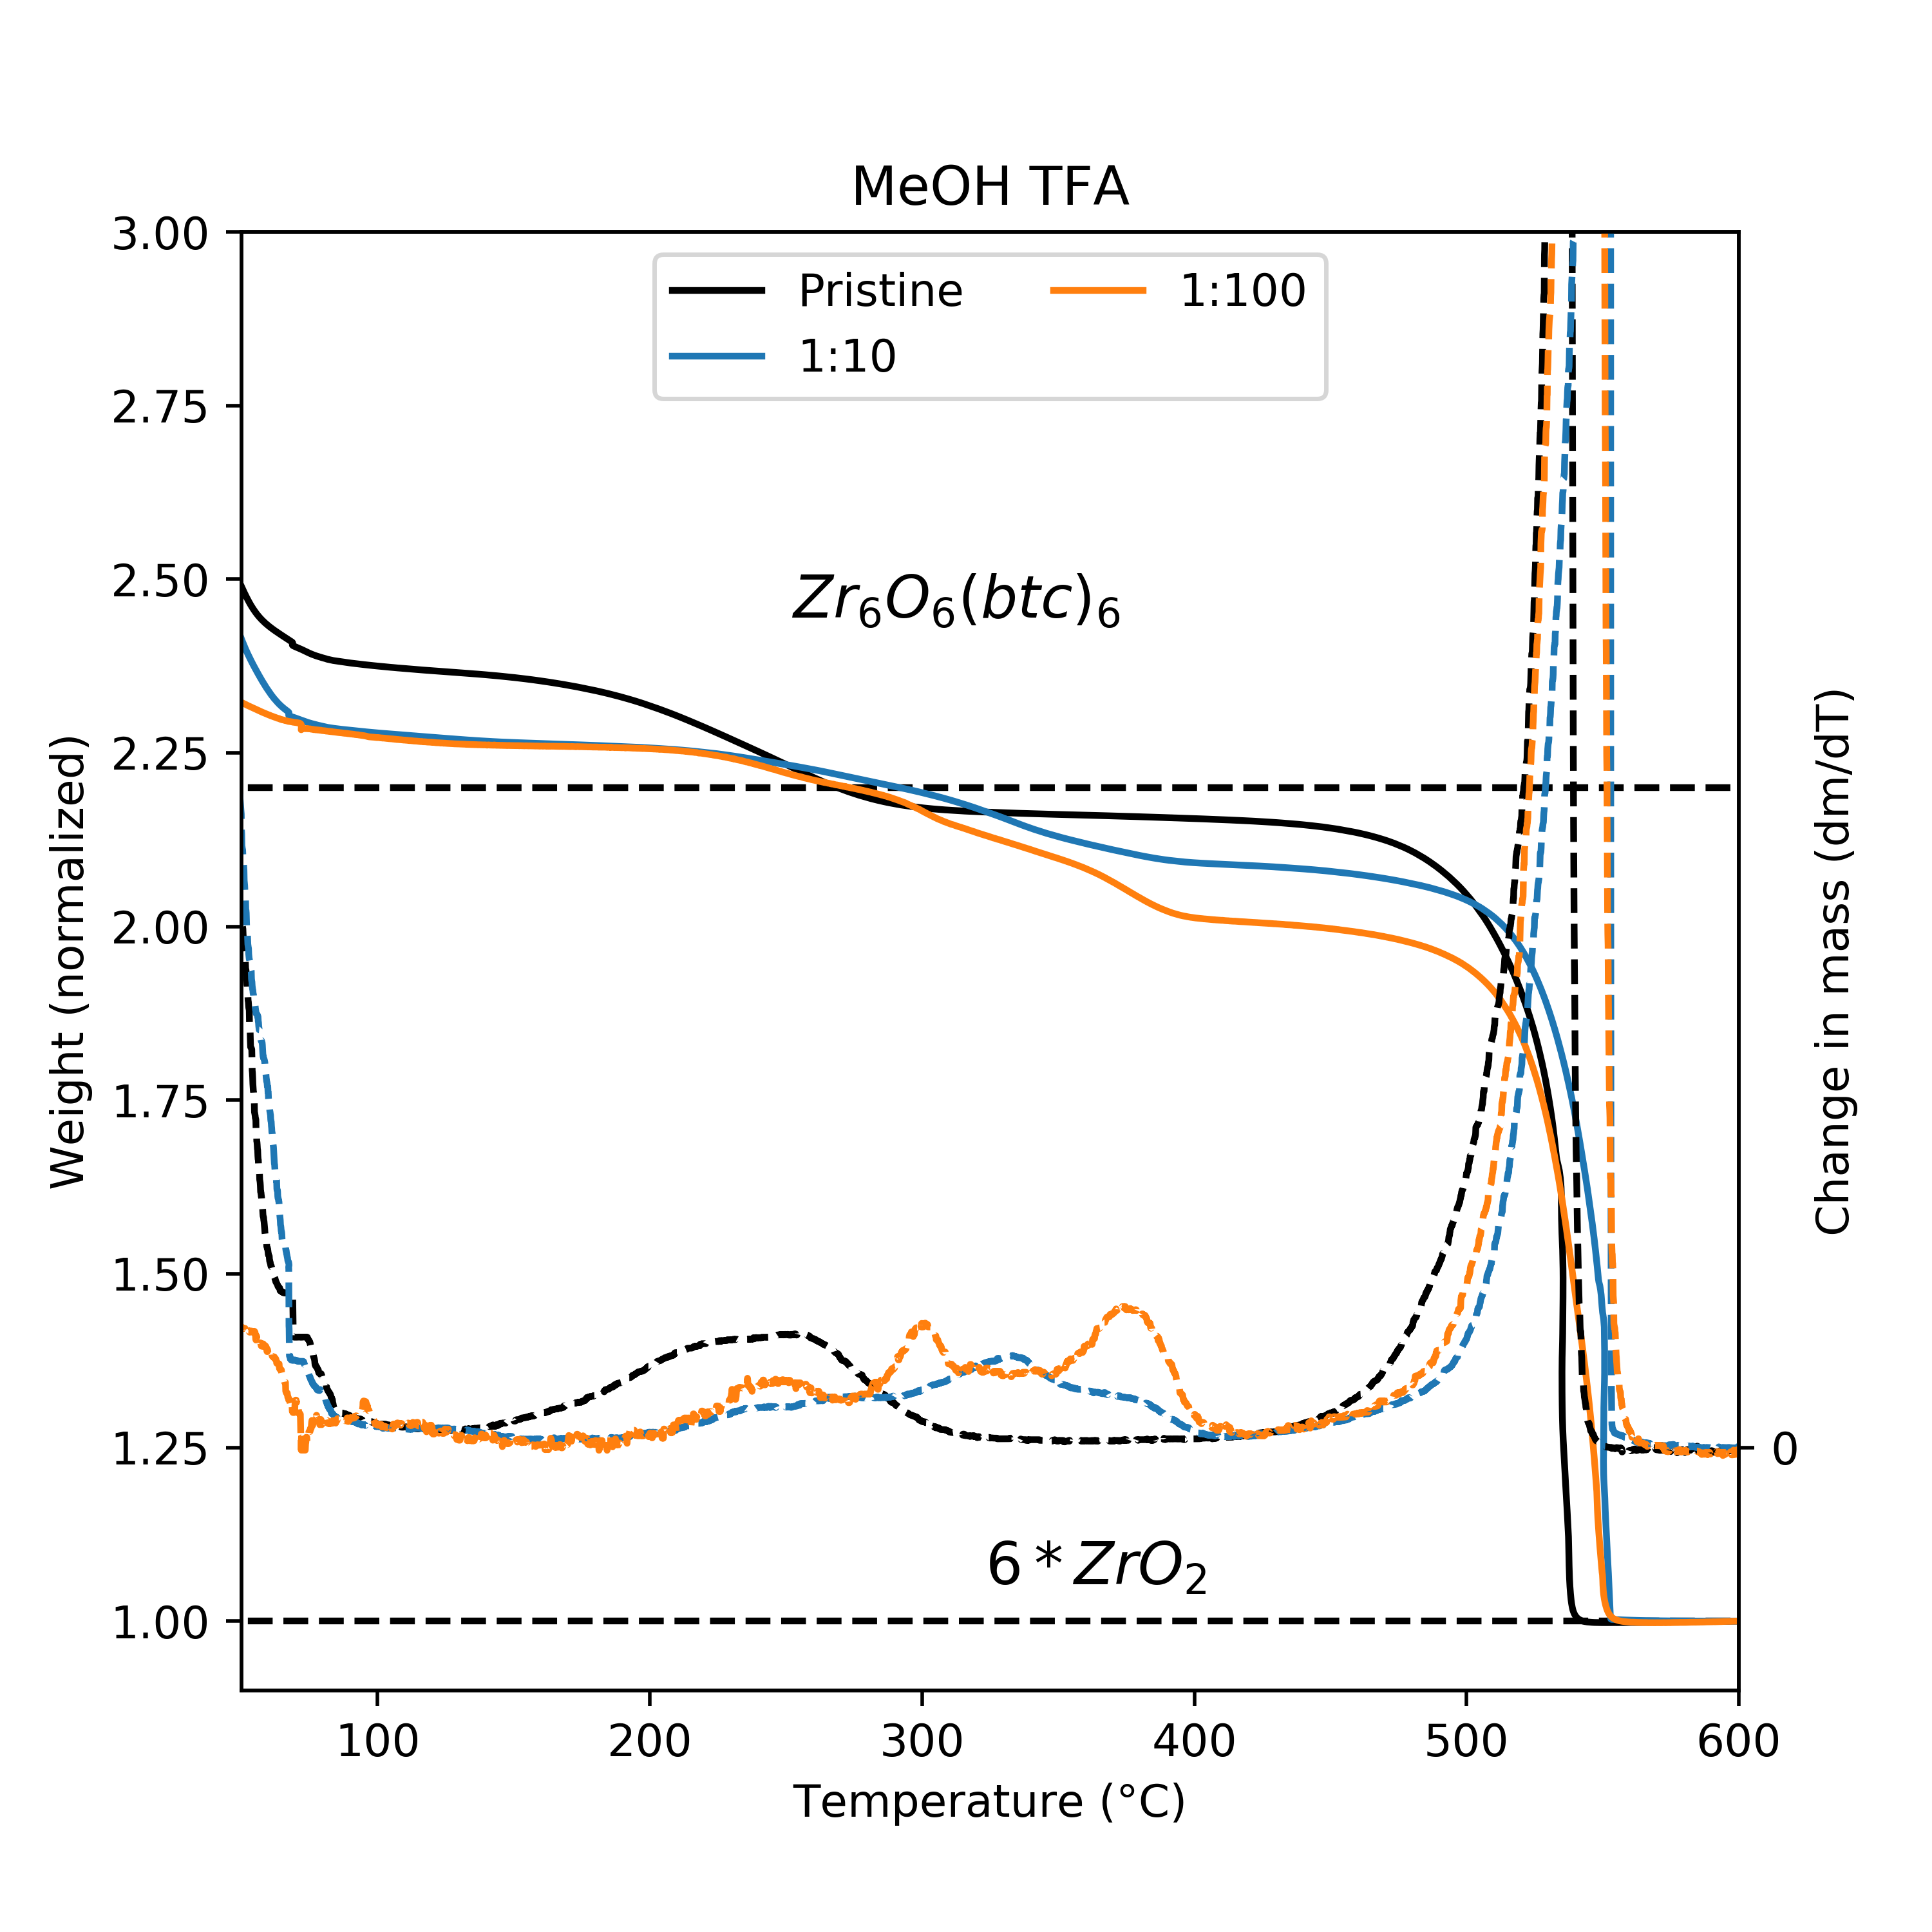
\includegraphics[width=\textwidth]{tga/MeOH-TFA}%
        \label{appx:def:fgr:tga-meoh-tfa}
    \end{subfigure}%
    \begin{subfigure}{0.4\linewidth}
        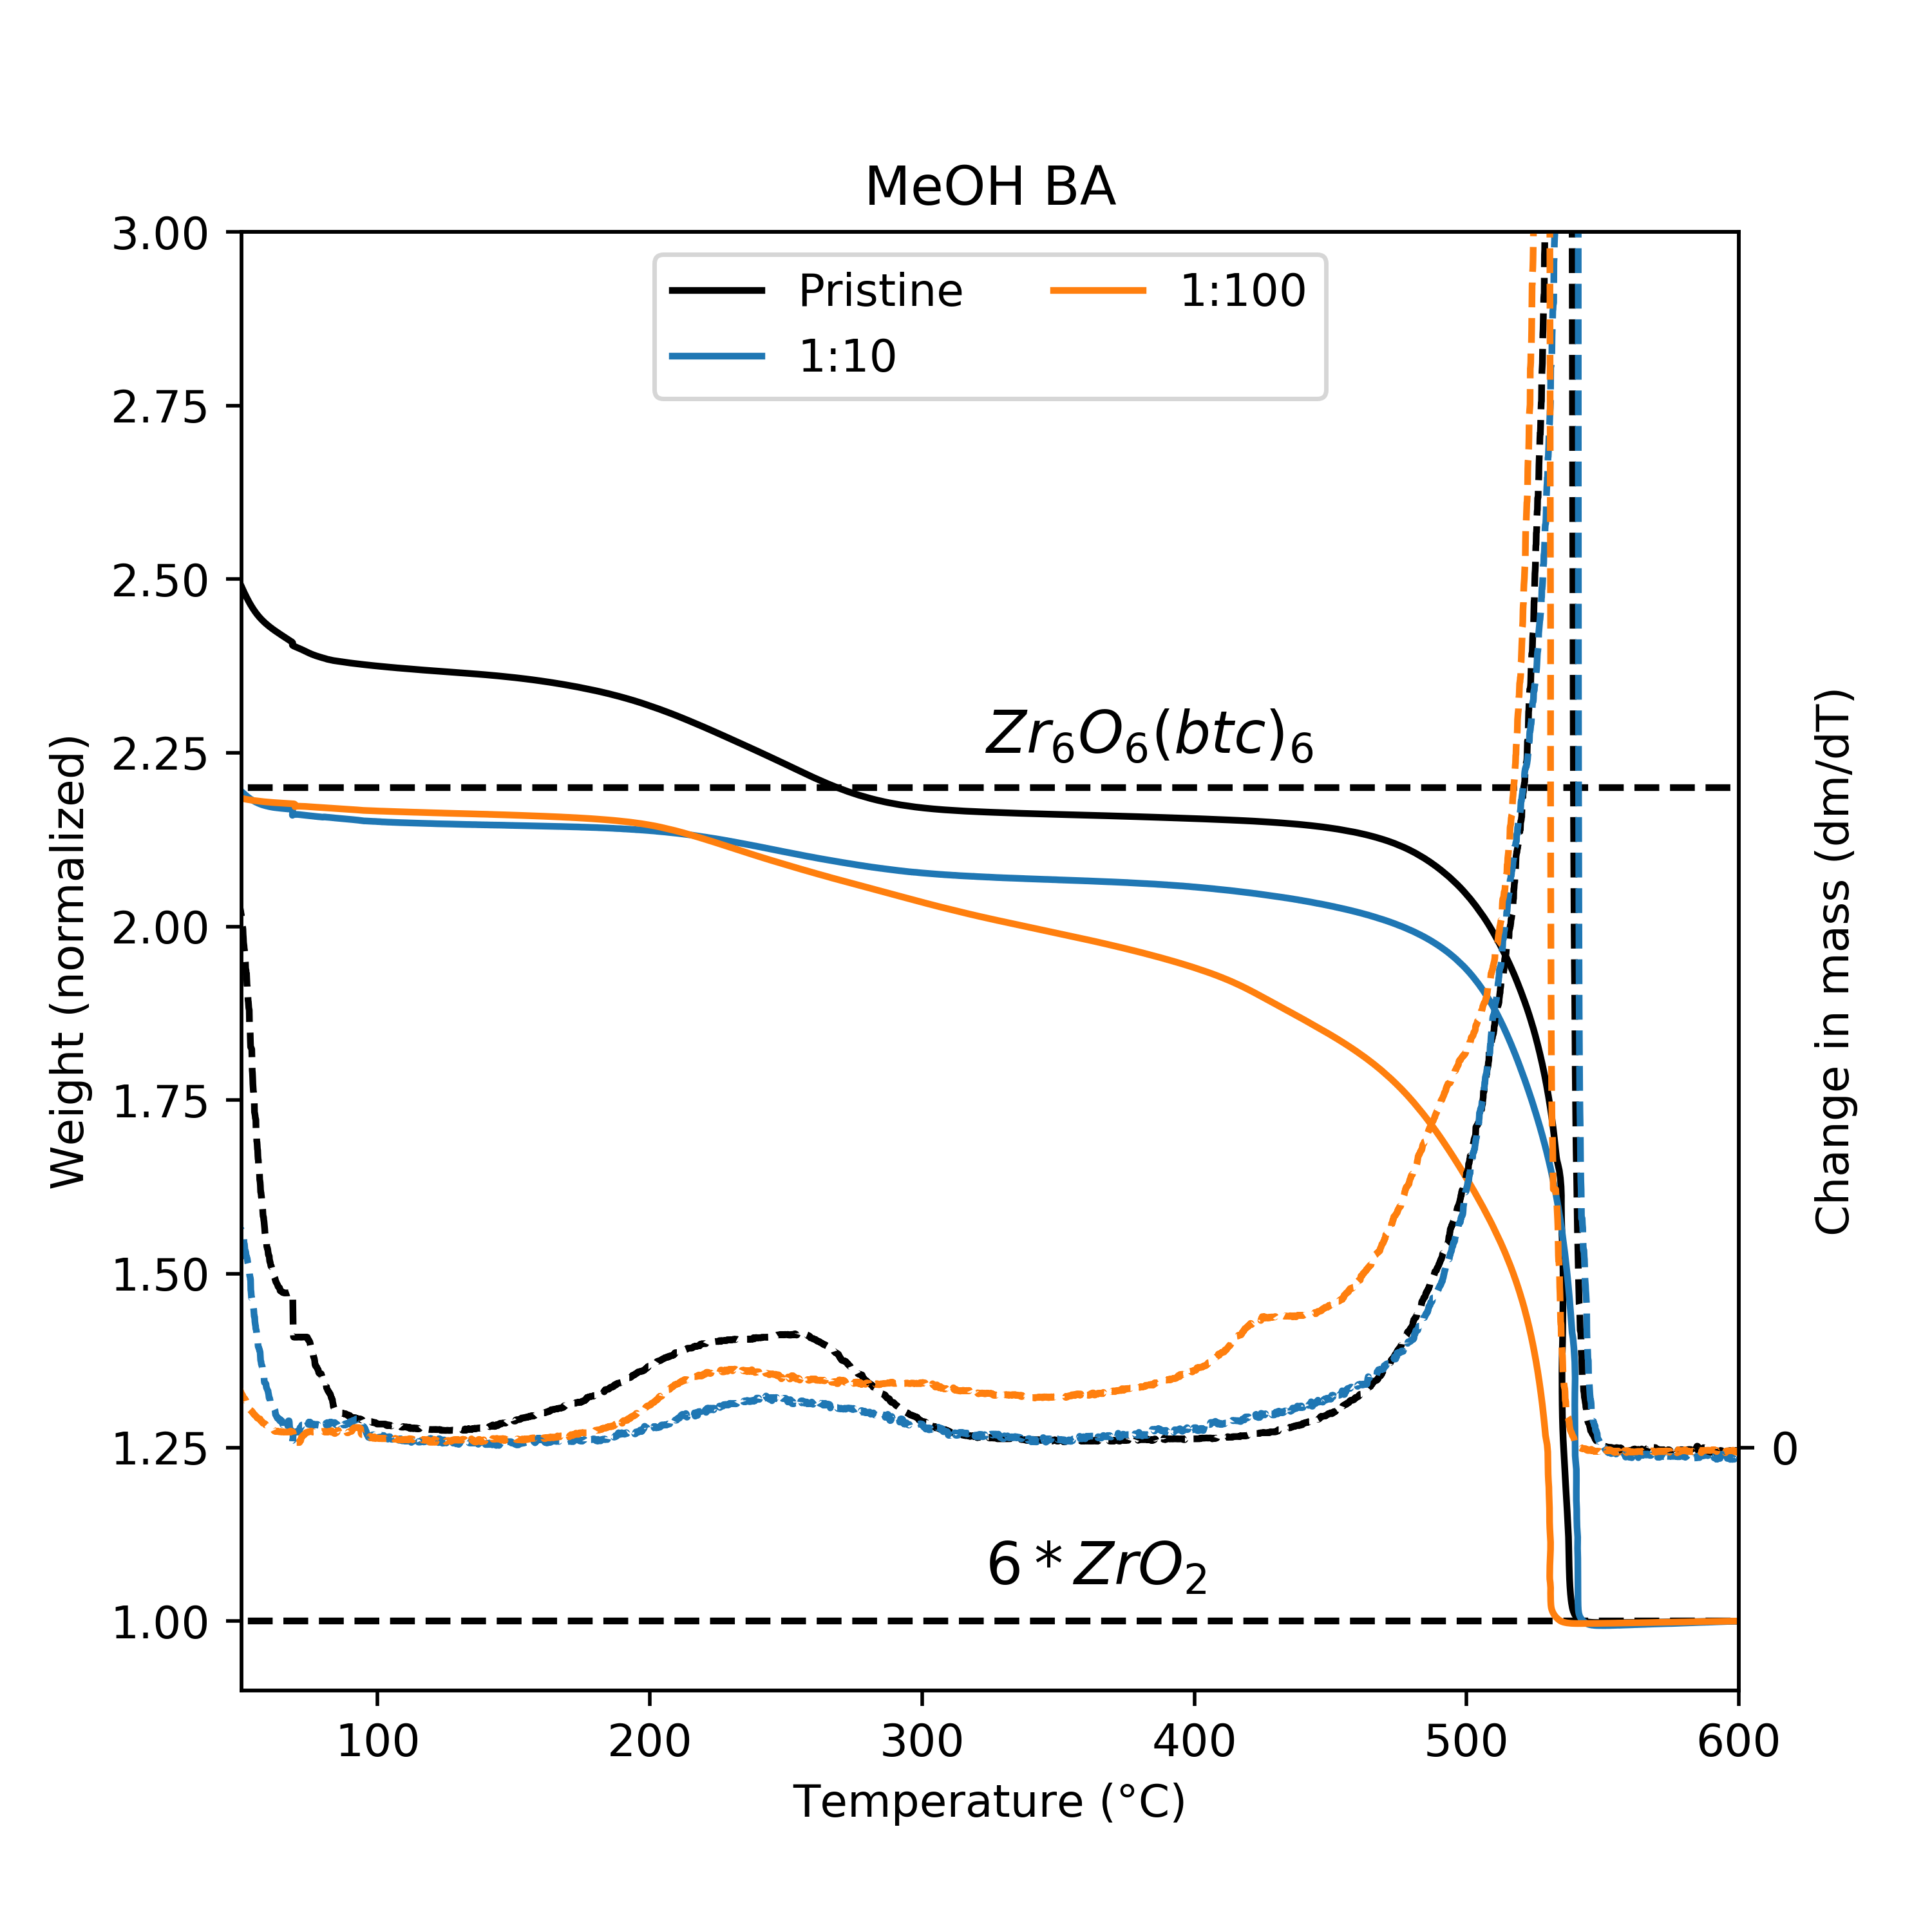
\includegraphics[width=\textwidth]{tga/MeOH-BA}%
        \label{appx:def:fgr:tga-meoh-ba}
    \end{subfigure}%

    \caption{TGA curves for samples leached in MeOH}%
\end{figure}

\FloatBarrier%
\pagebreak
\subsection{DMSO leached samples}
\begin{figure}[!h]
    \centering

    \begin{subfigure}{0.4\linewidth}
        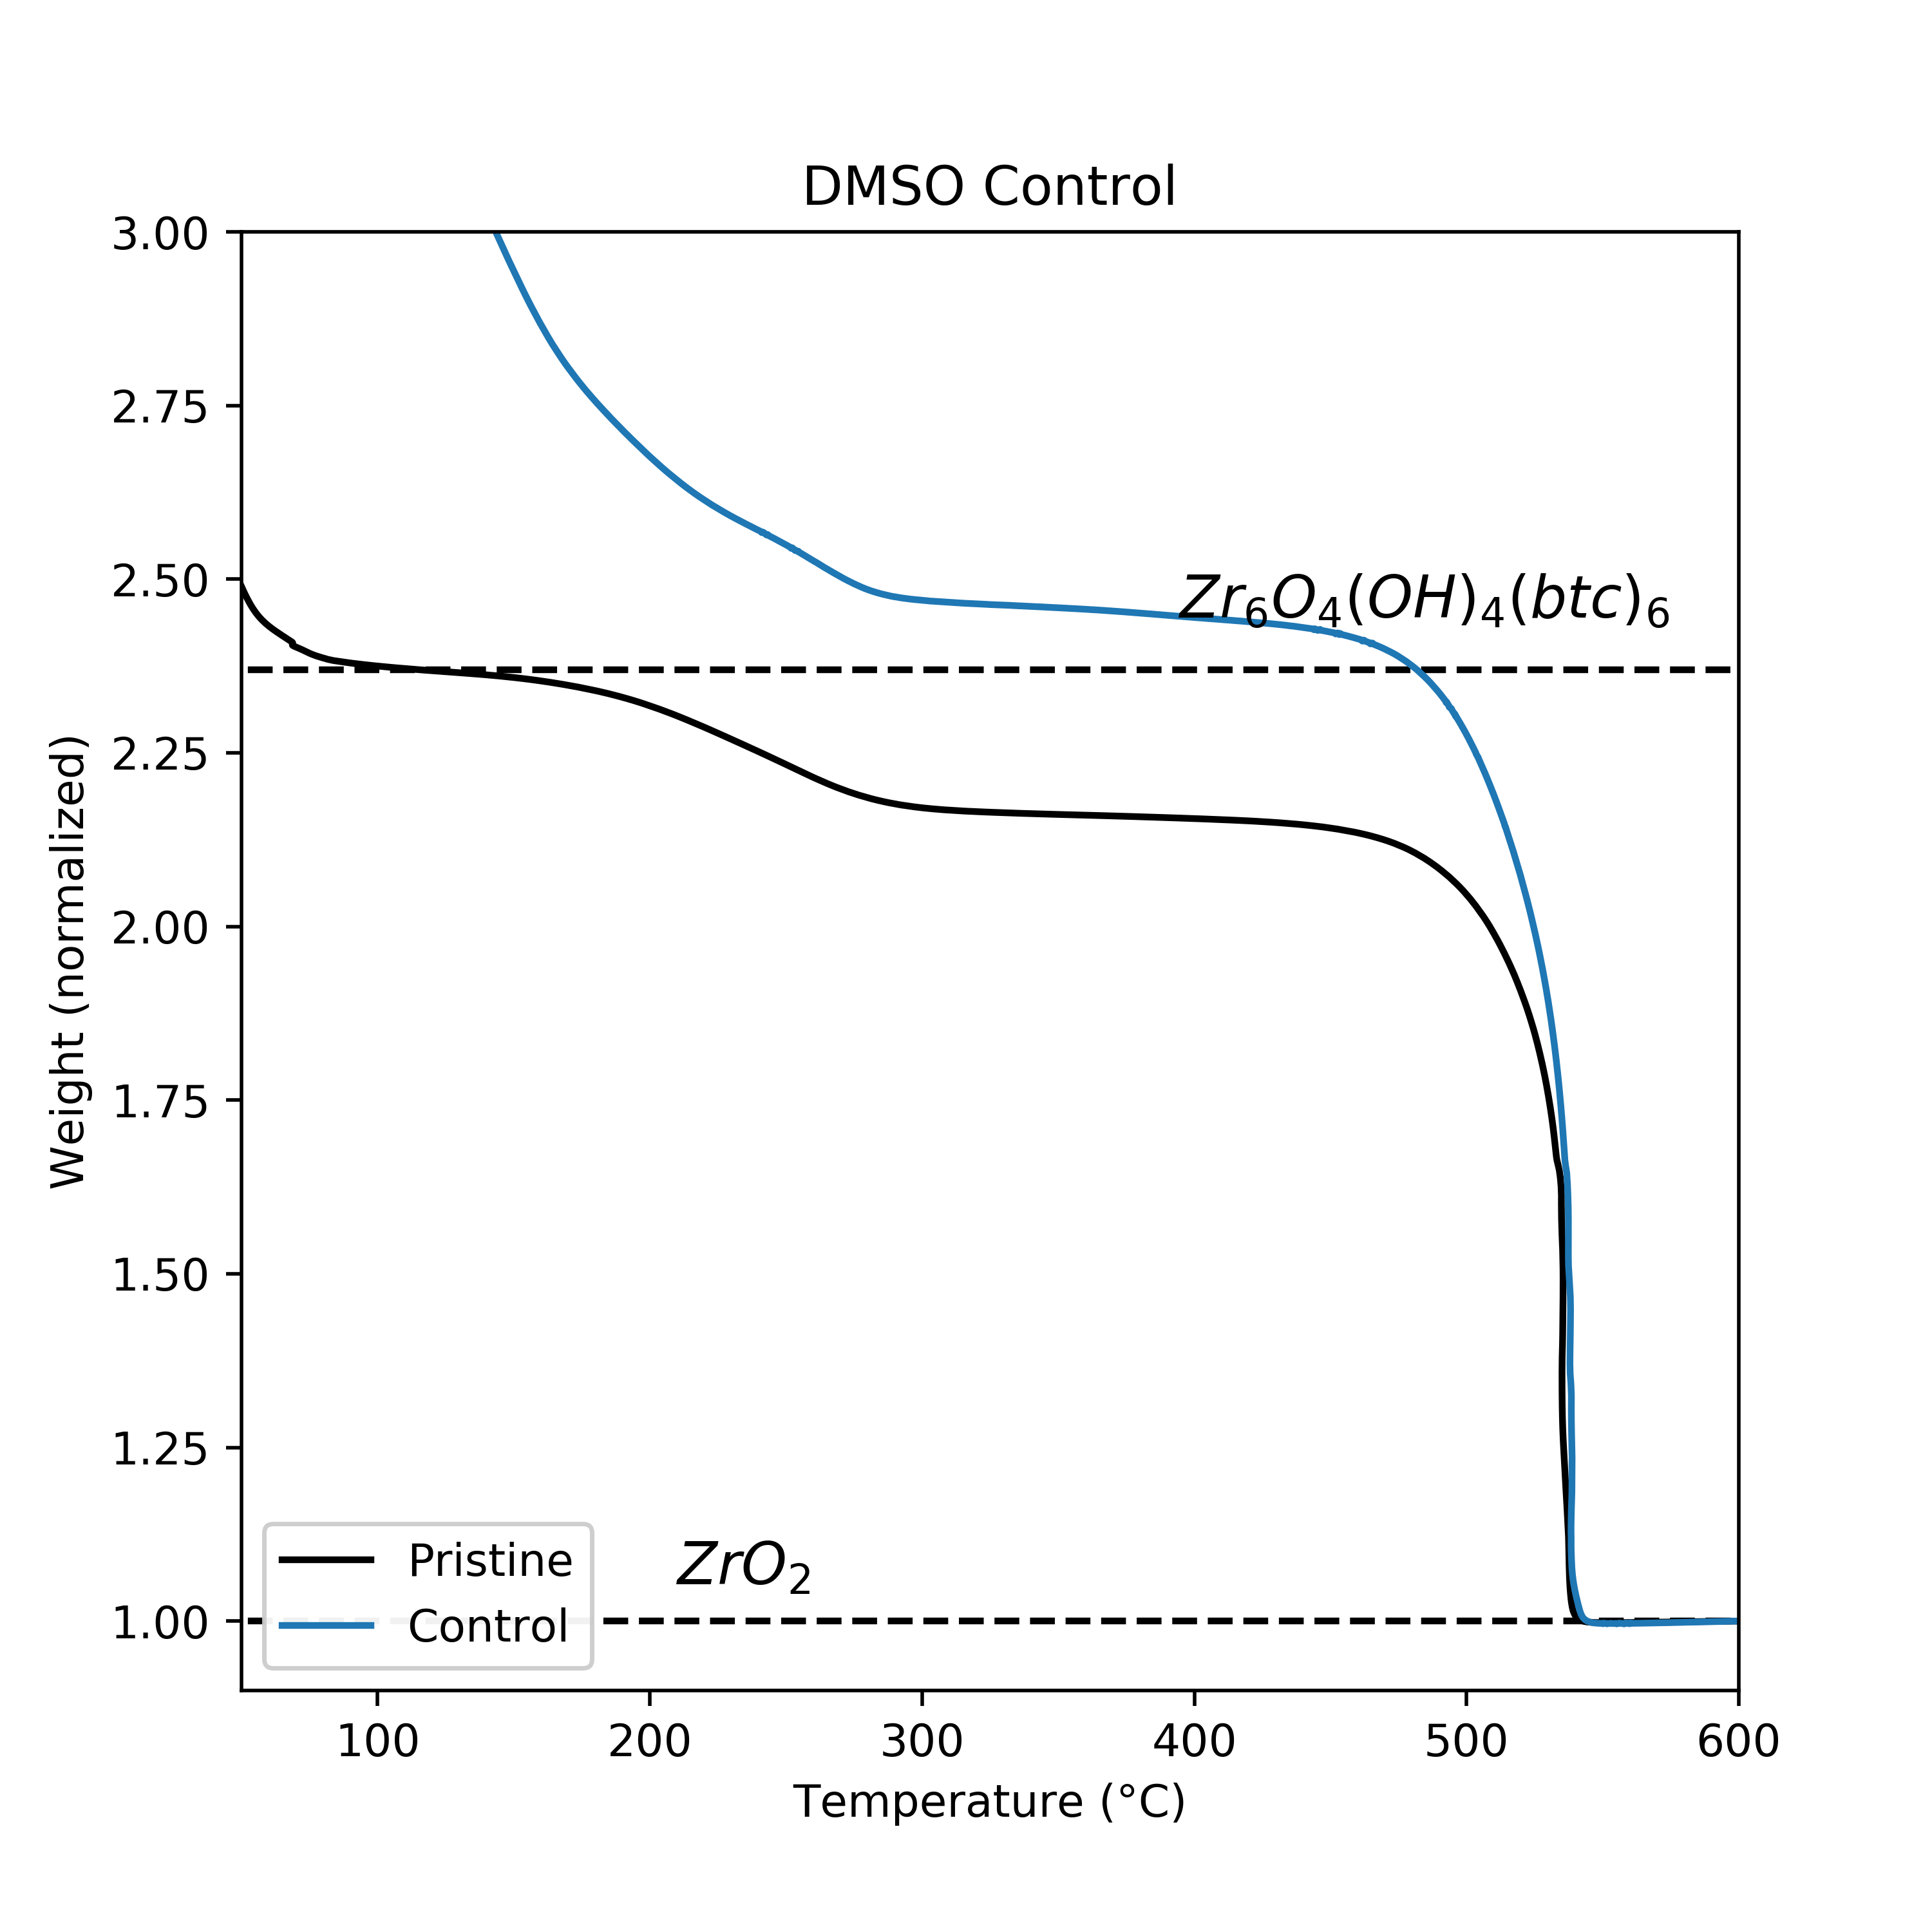
\includegraphics[width=\textwidth]{tga/DMSO-Control}%
        \label{appx:def:fgr:tga-dmso-cont}
    \end{subfigure}%

    \begin{subfigure}{0.4\linewidth}
        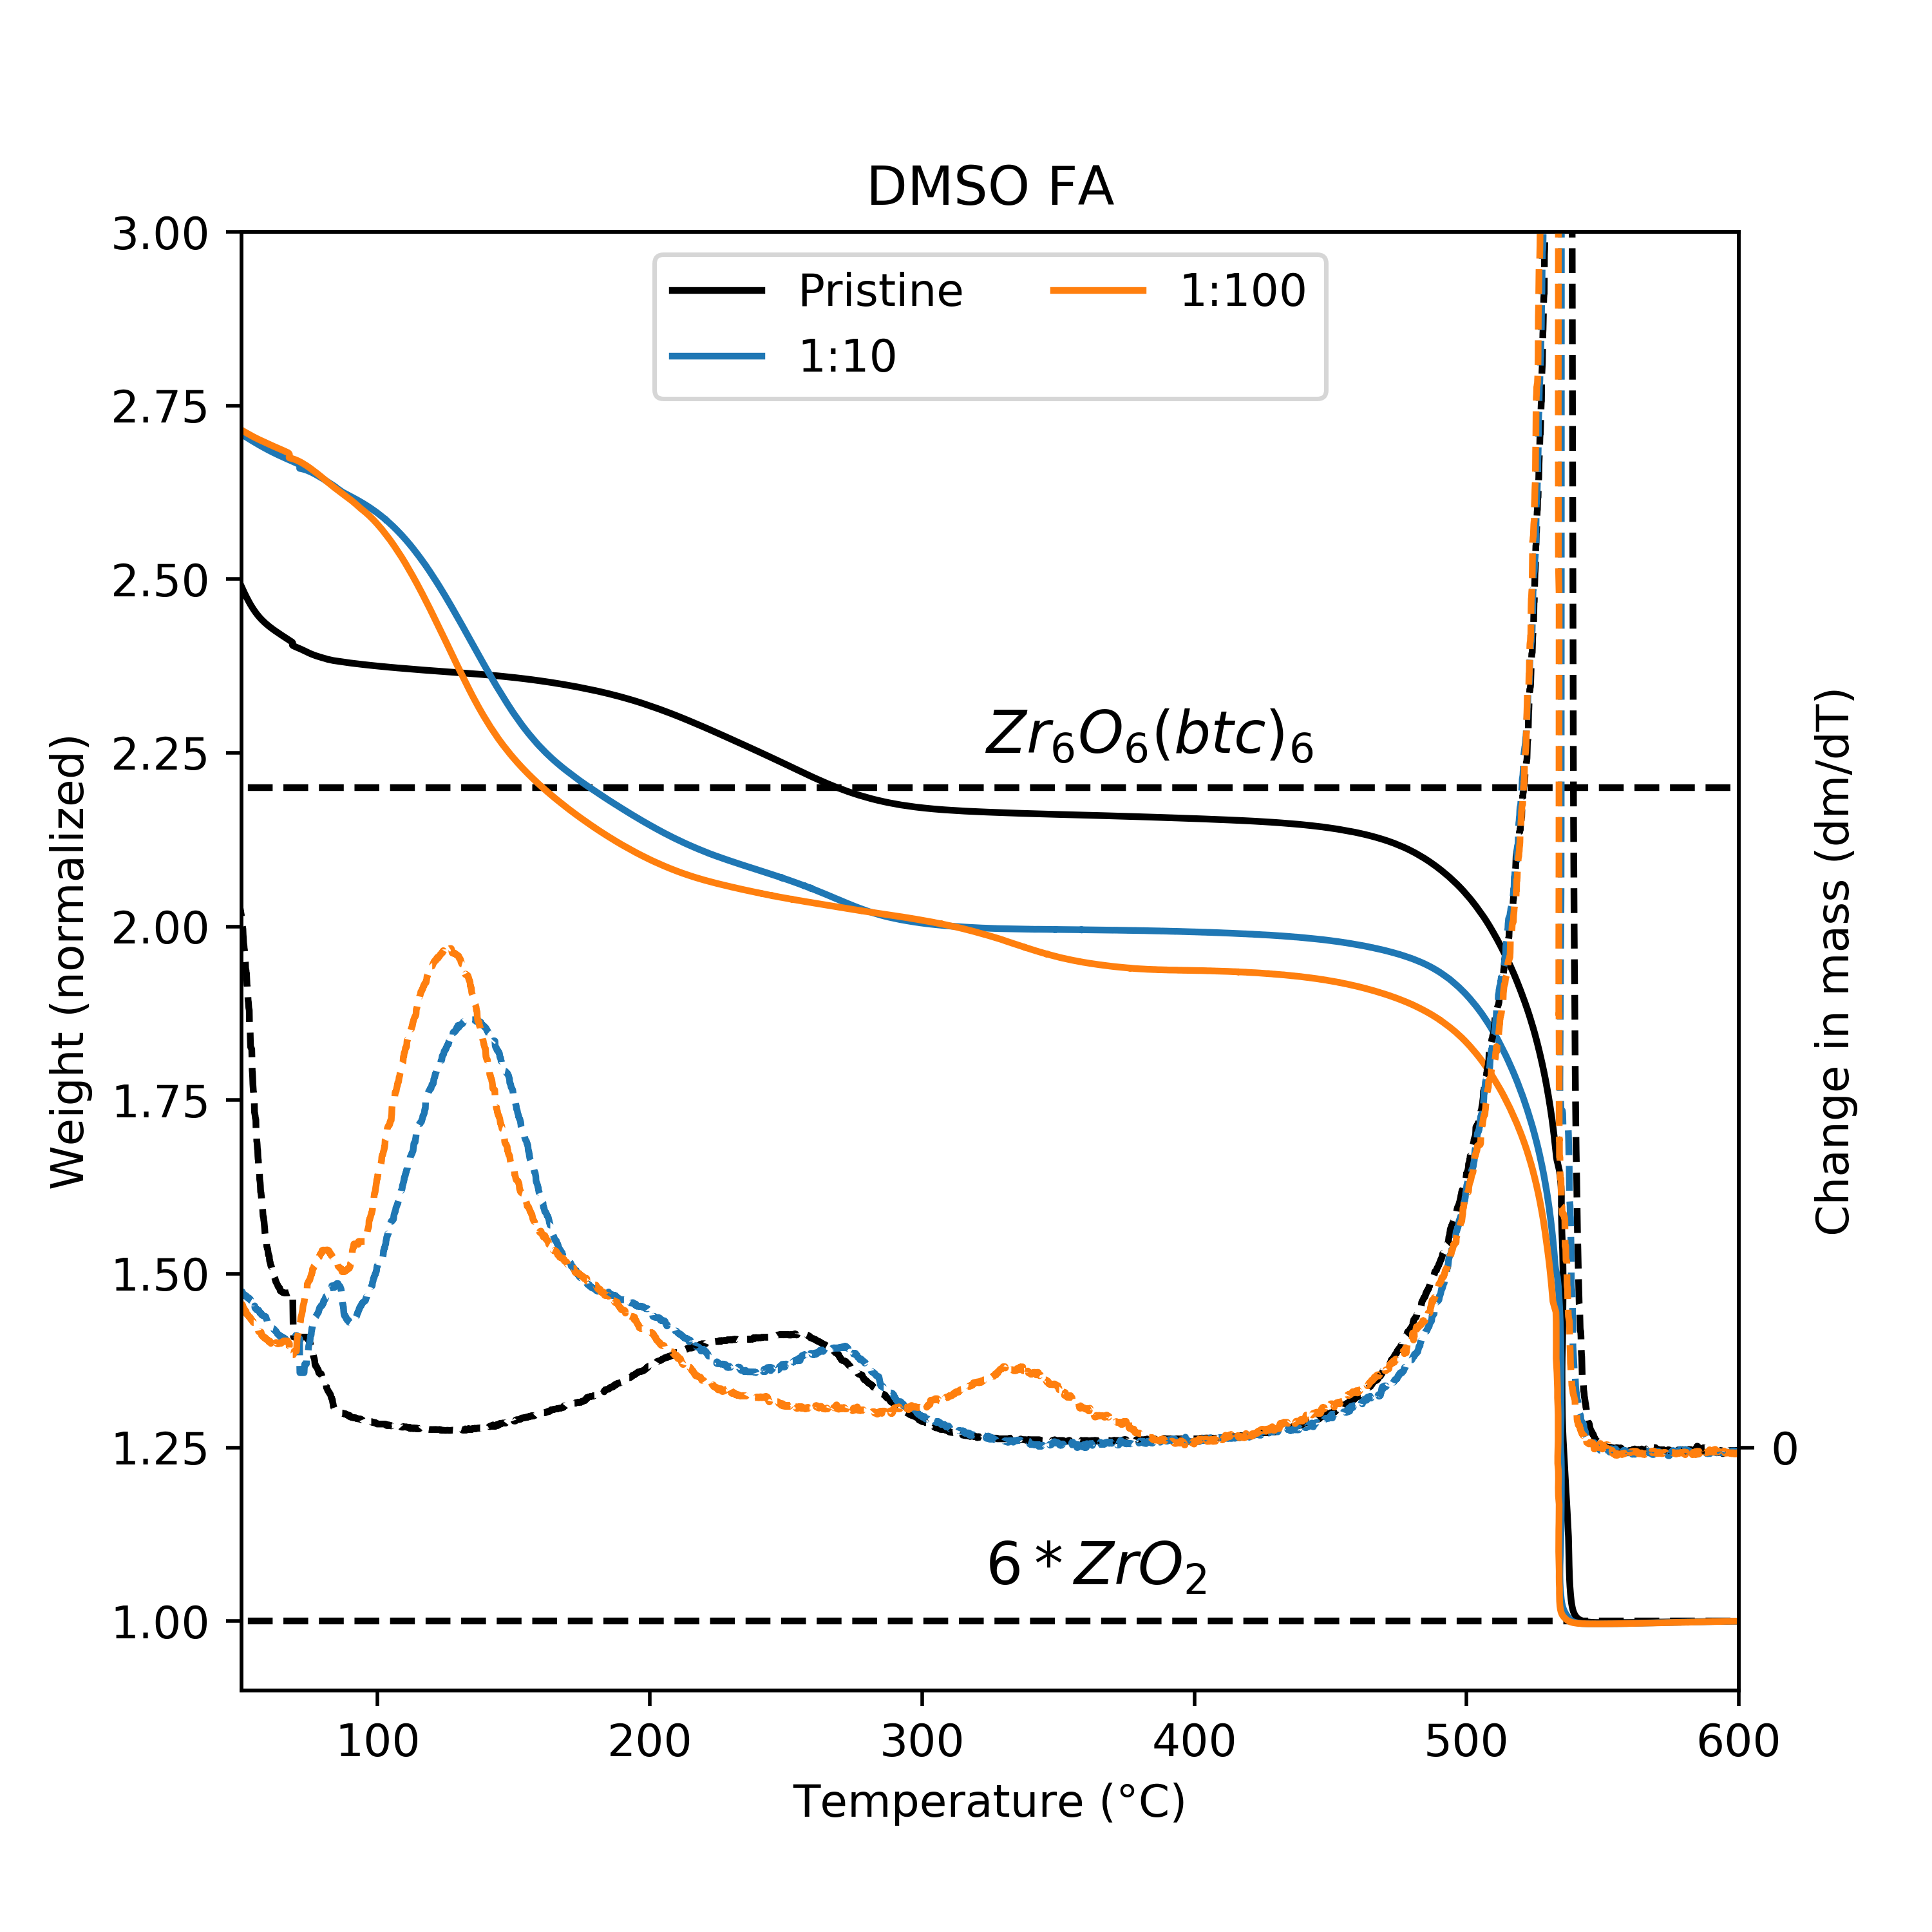
\includegraphics[width=\textwidth]{tga/DMSO-FA}%
        \label{appx:def:fgr:tga-dmso-fa}
    \end{subfigure}%
    \begin{subfigure}{0.4\linewidth}
        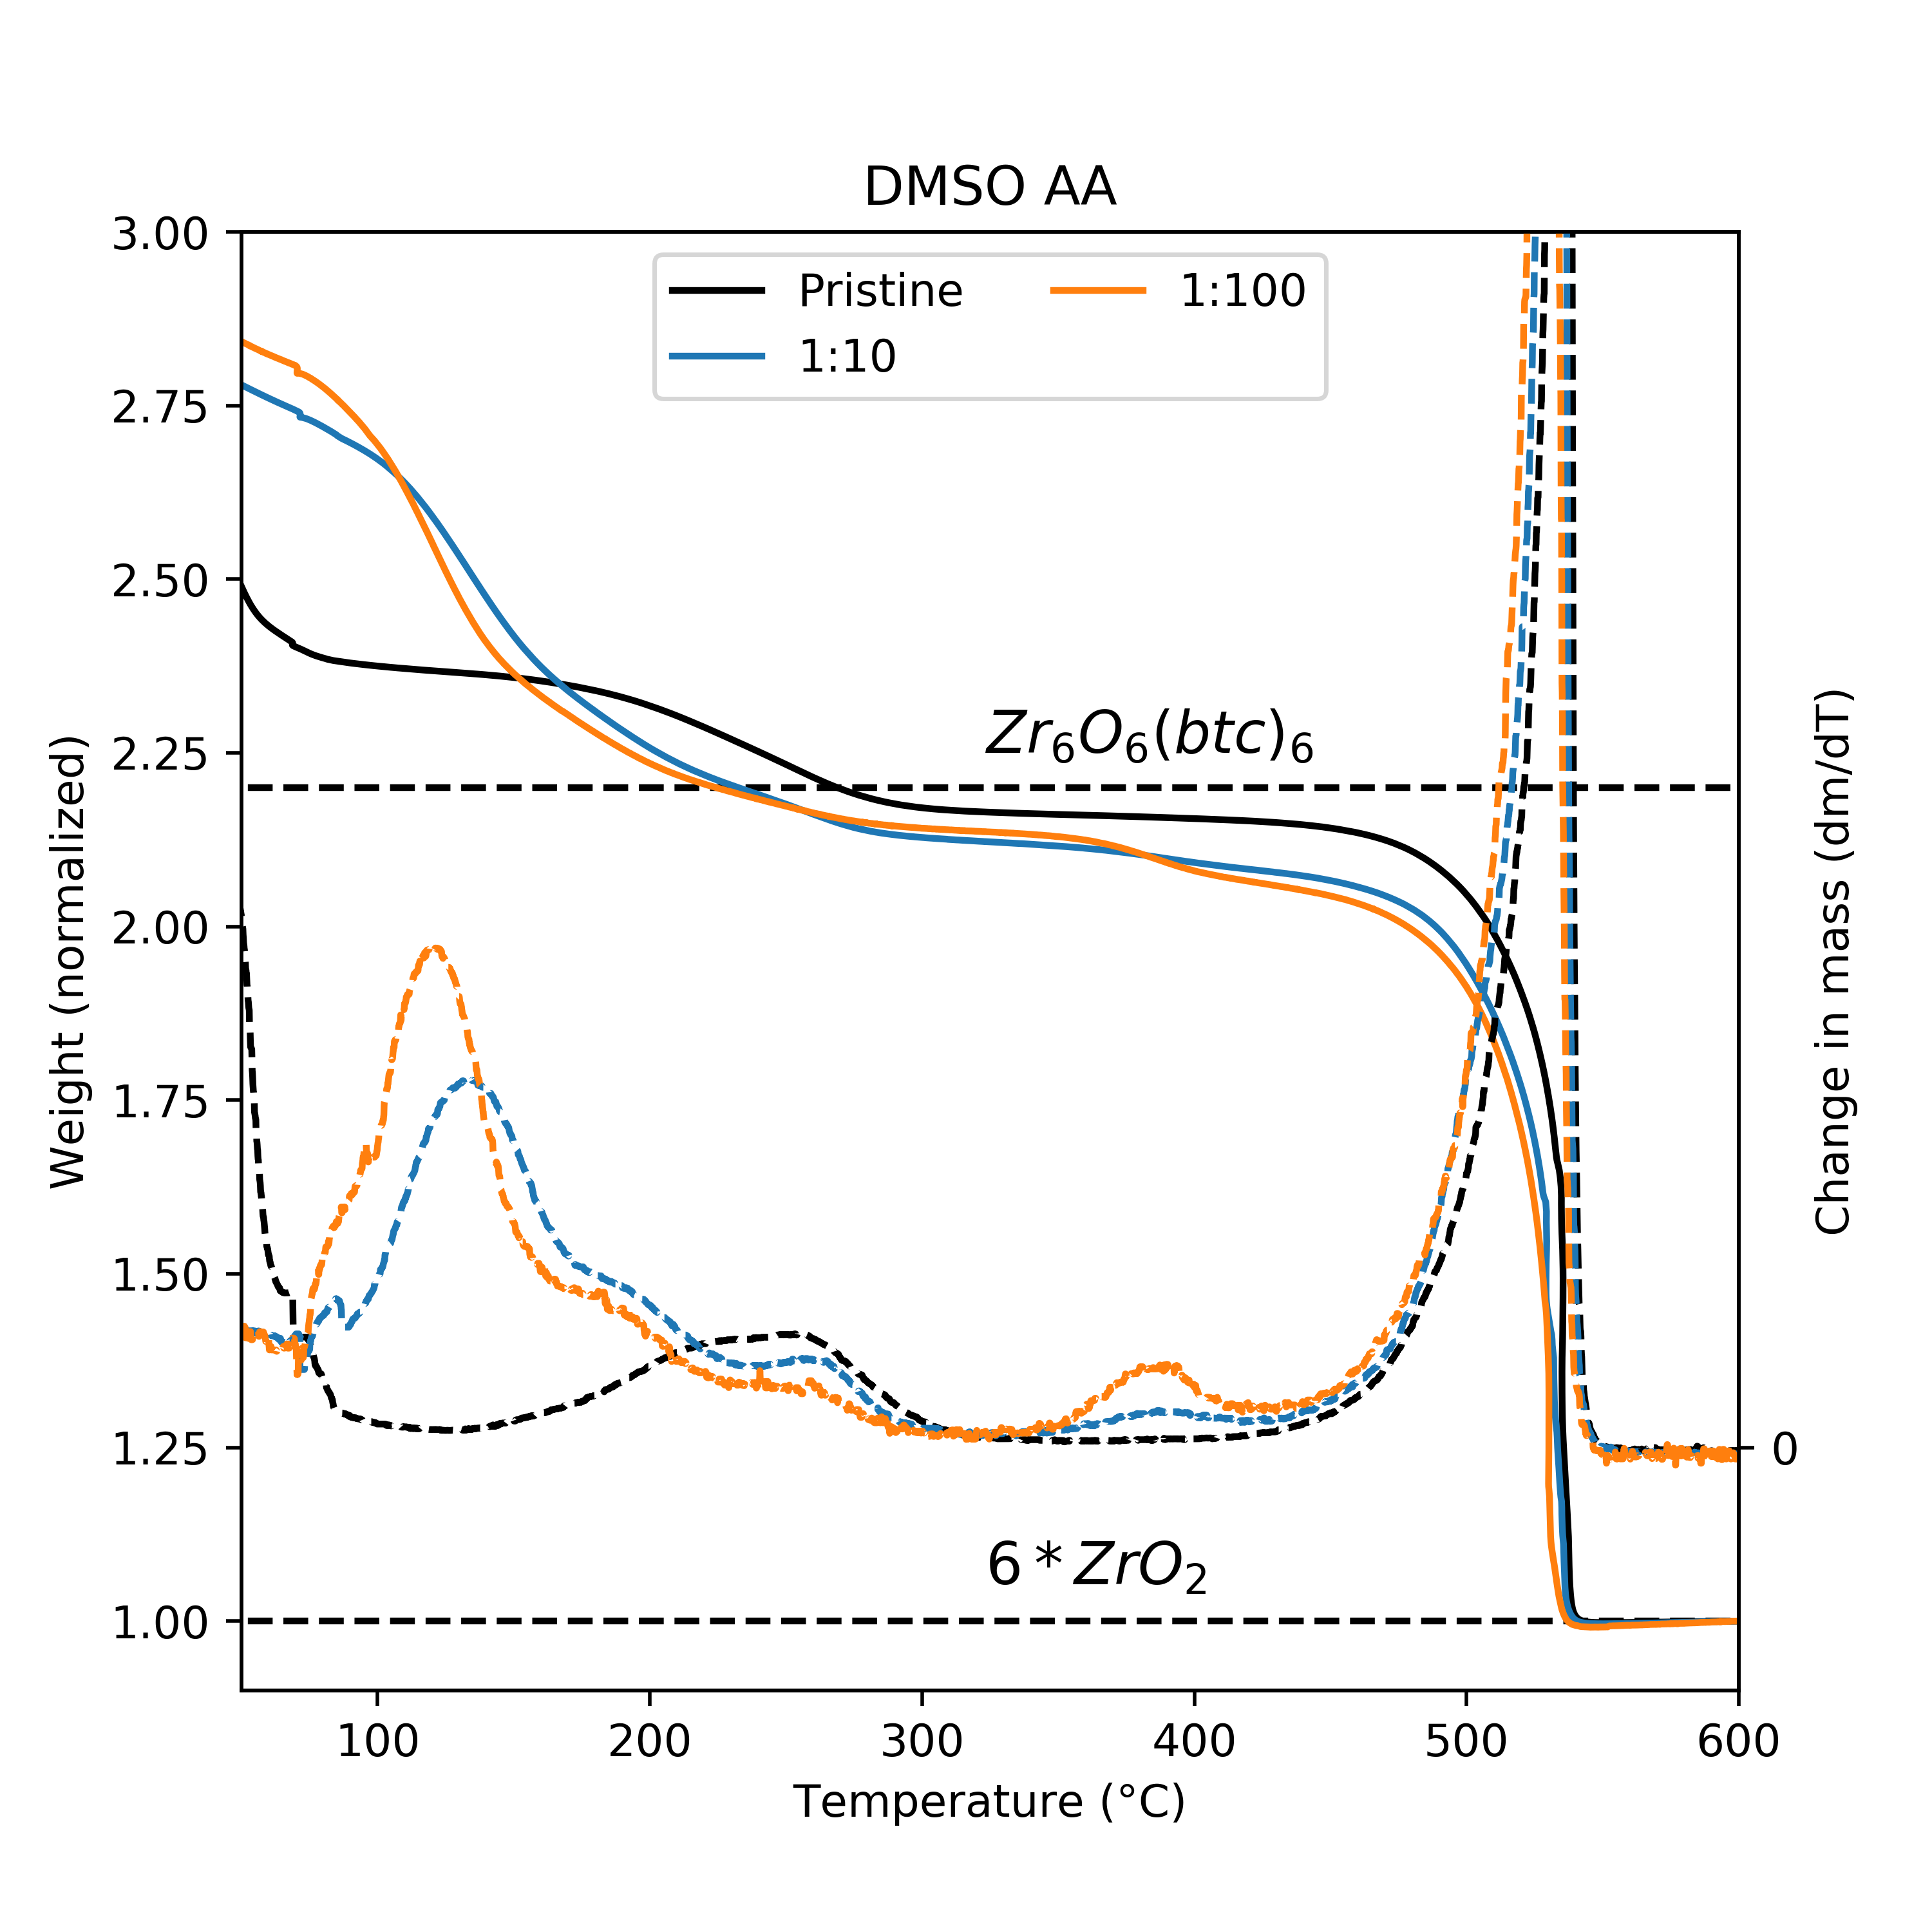
\includegraphics[width=\textwidth]{tga/DMSO-AA}%
        \label{appx:def:fgr:tga-dmso-aa}
    \end{subfigure}%

    \begin{subfigure}{0.4\linewidth}
        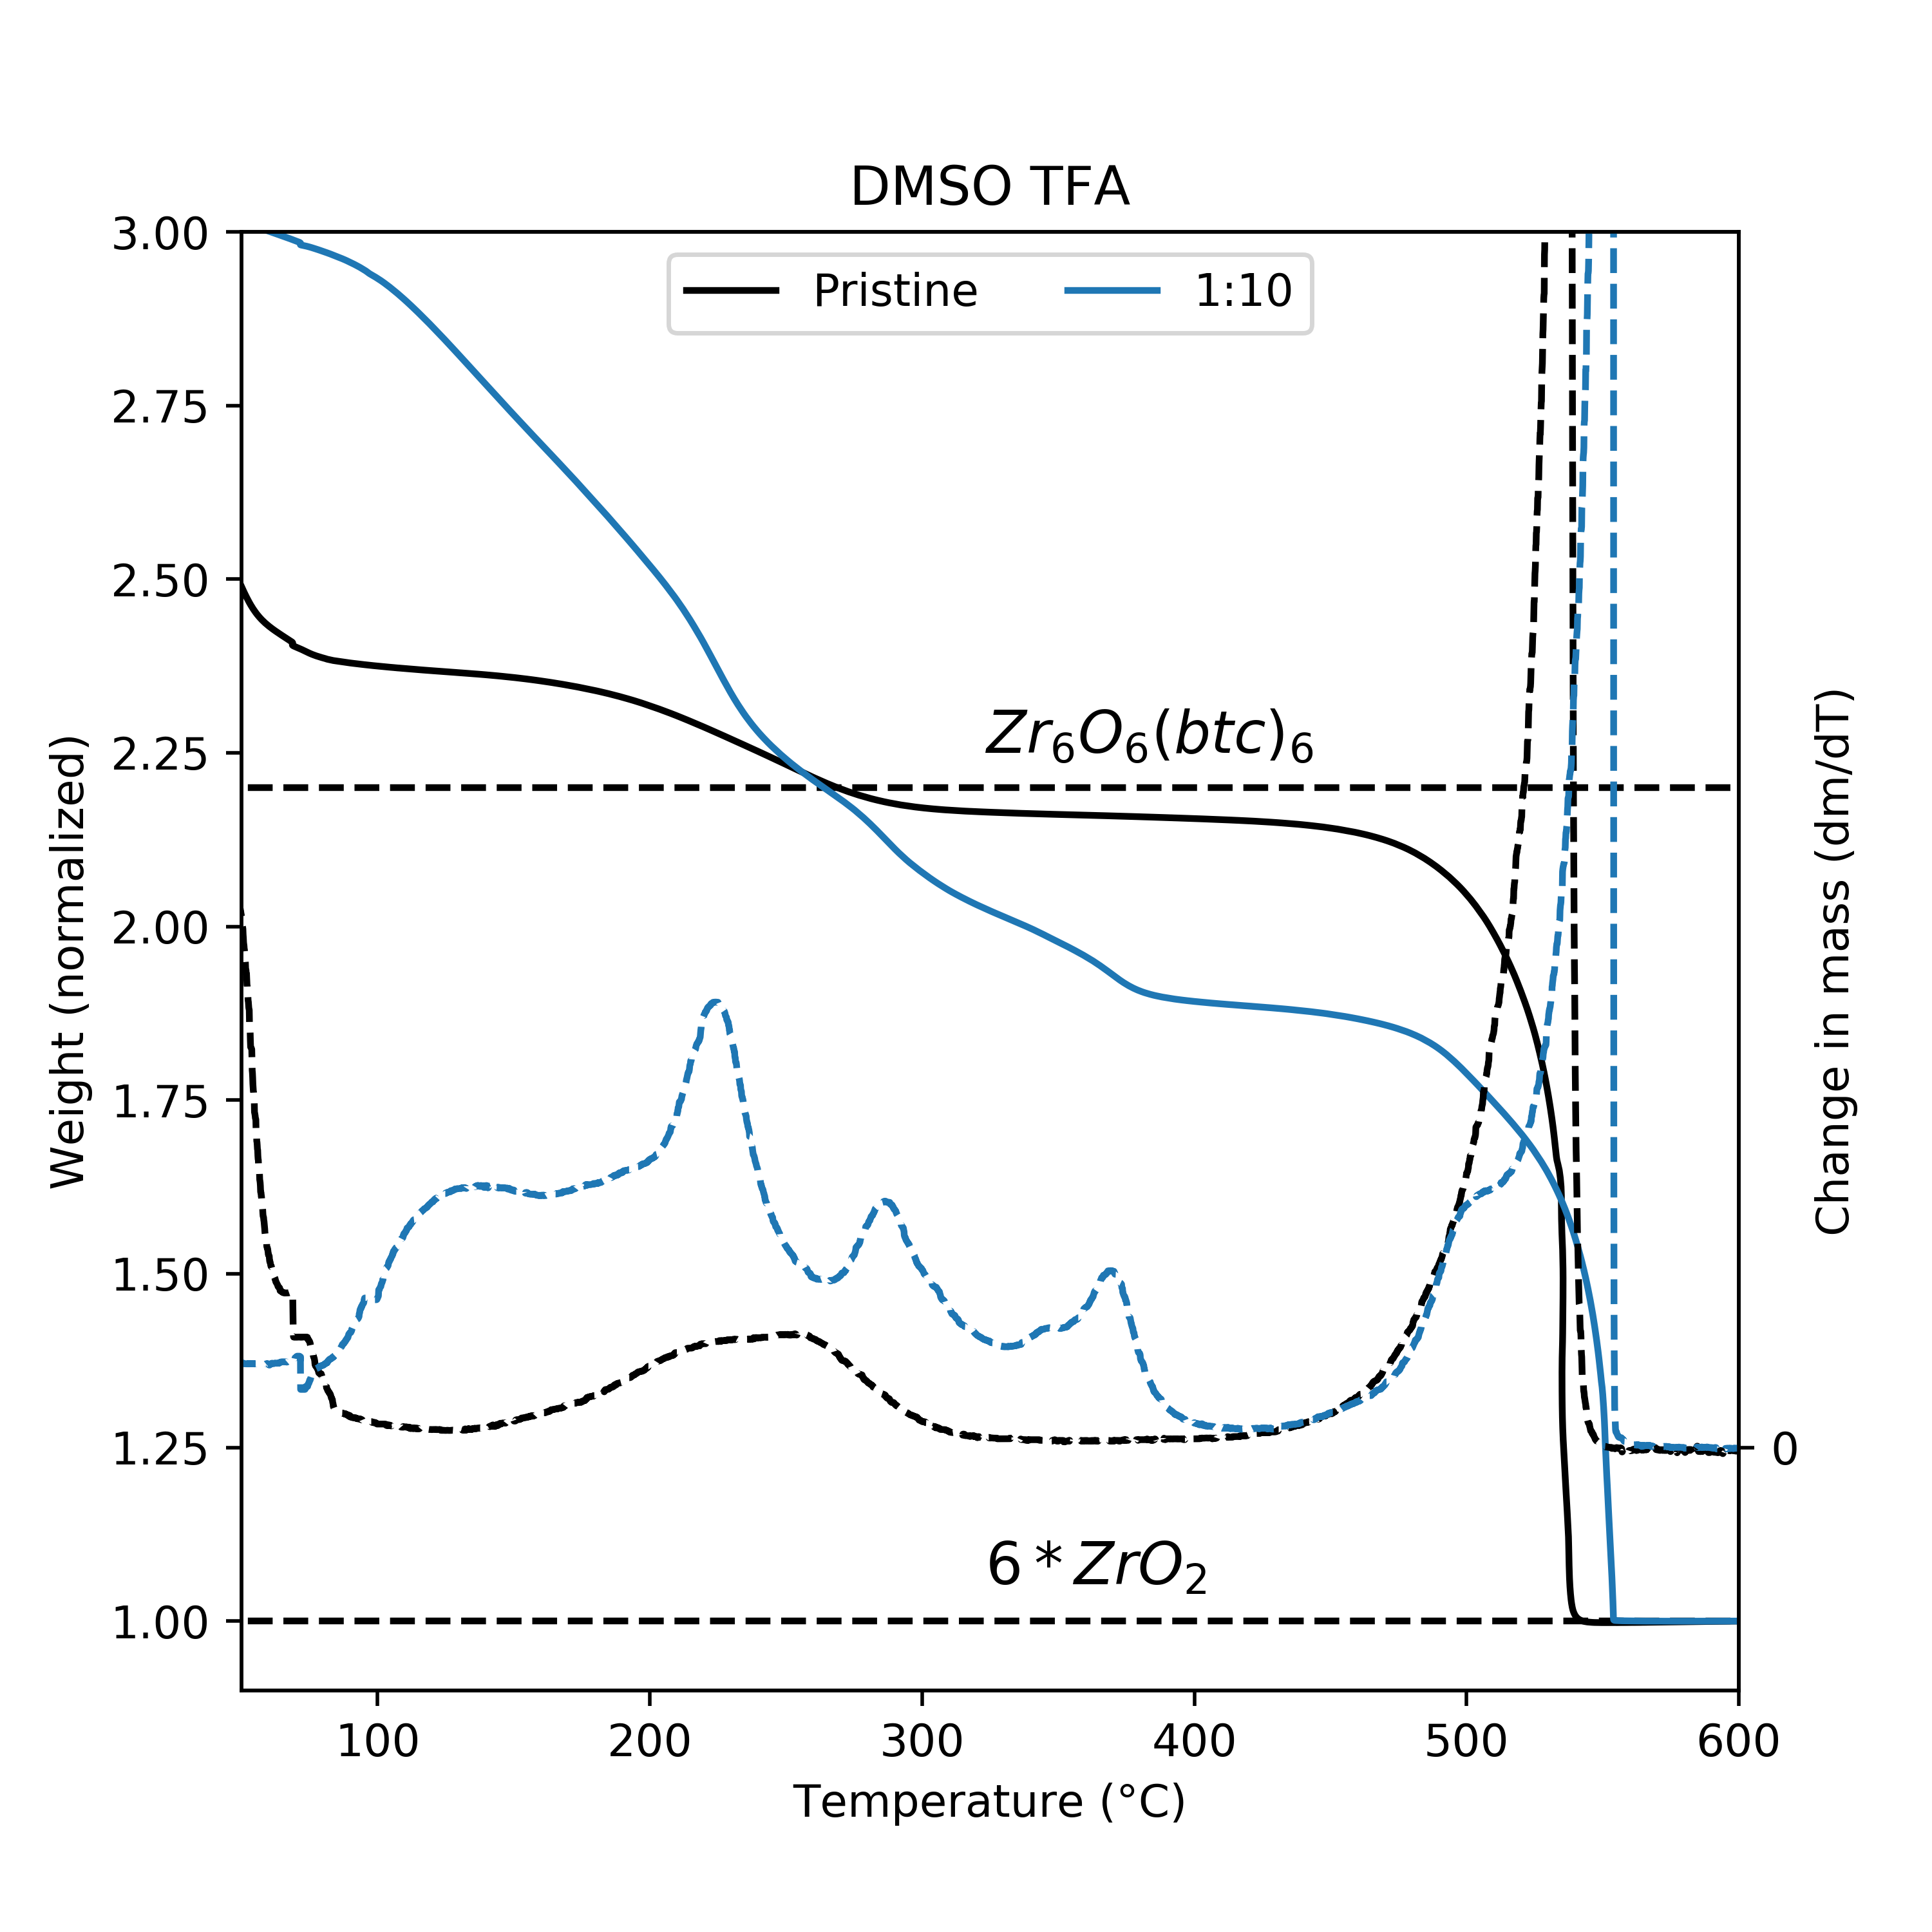
\includegraphics[width=\textwidth]{tga/DMSO-TFA}%
        \label{appx:def:fgr:tga-dmso-tfa}
    \end{subfigure}%
    \begin{subfigure}{0.4\linewidth}
        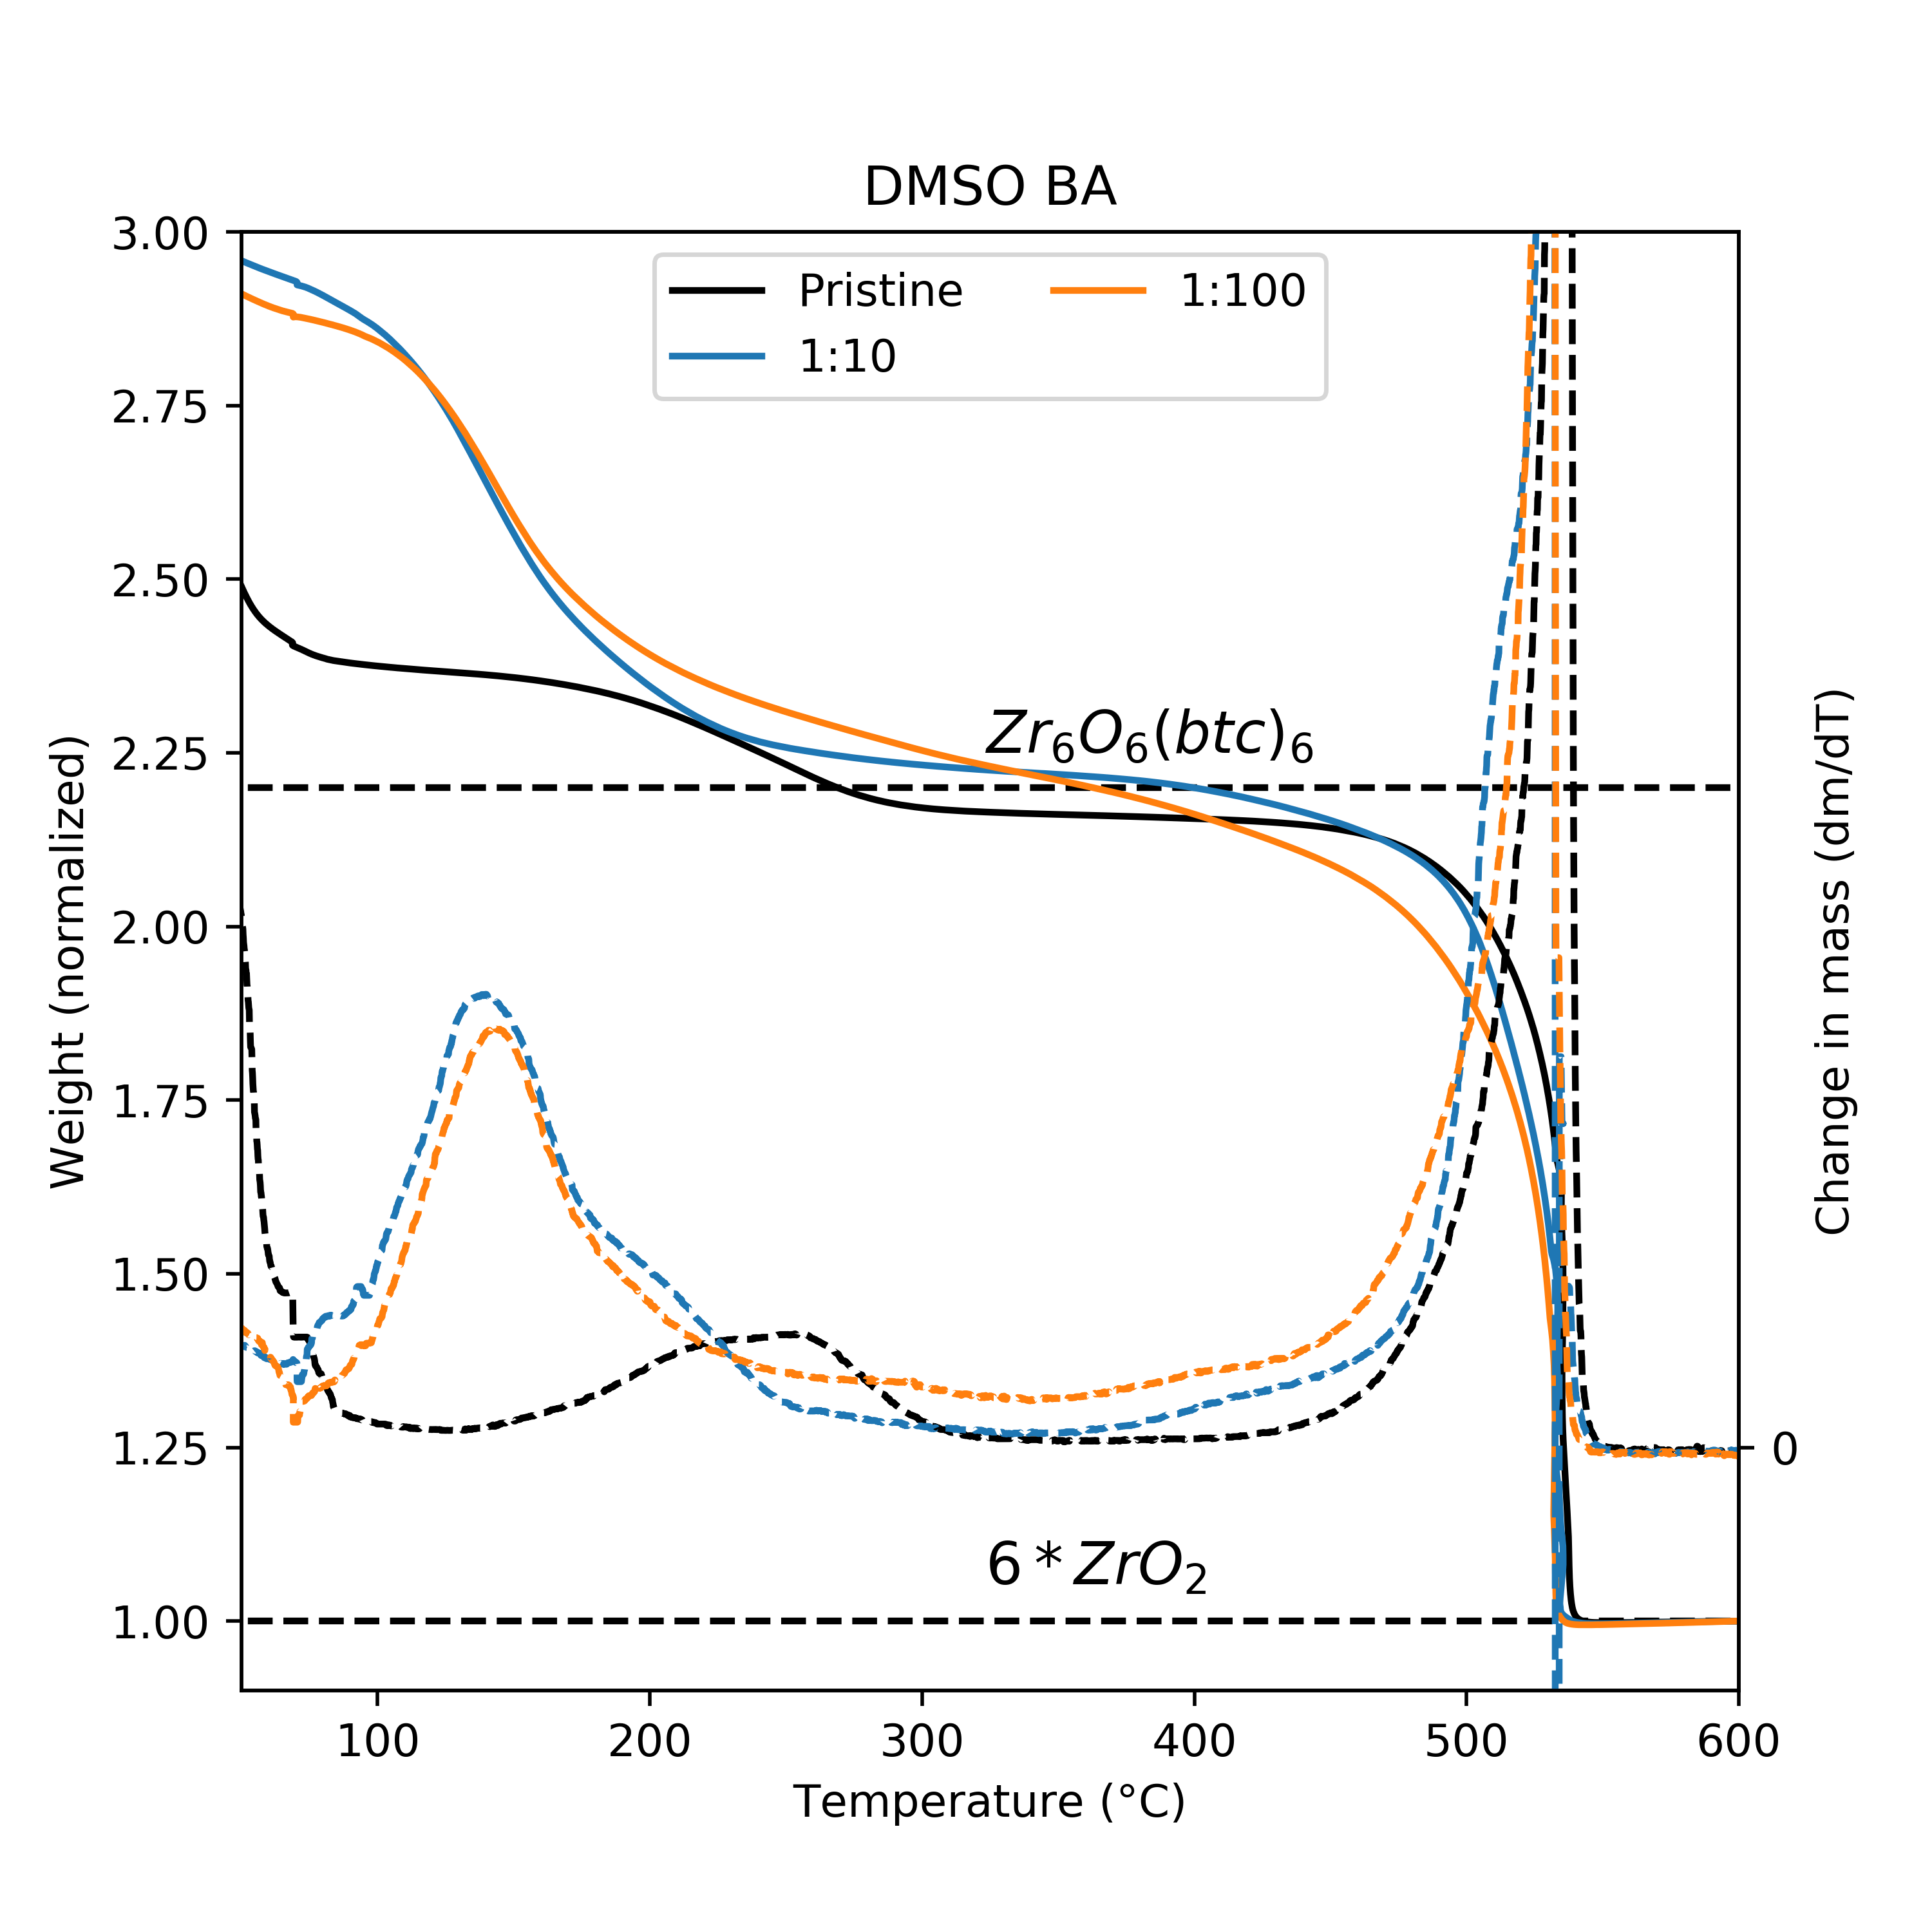
\includegraphics[width=\textwidth]{tga/DMSO-BA}%
        \label{appx:def:fgr:tga-dmso-ba}
    \end{subfigure}%

    \caption{TGA curves for samples leached in DMSO}%
\end{figure}

\FloatBarrier%
\pagebreak
\subsection{High resolution curves}

\begin{figure}[!h]

    \centering

    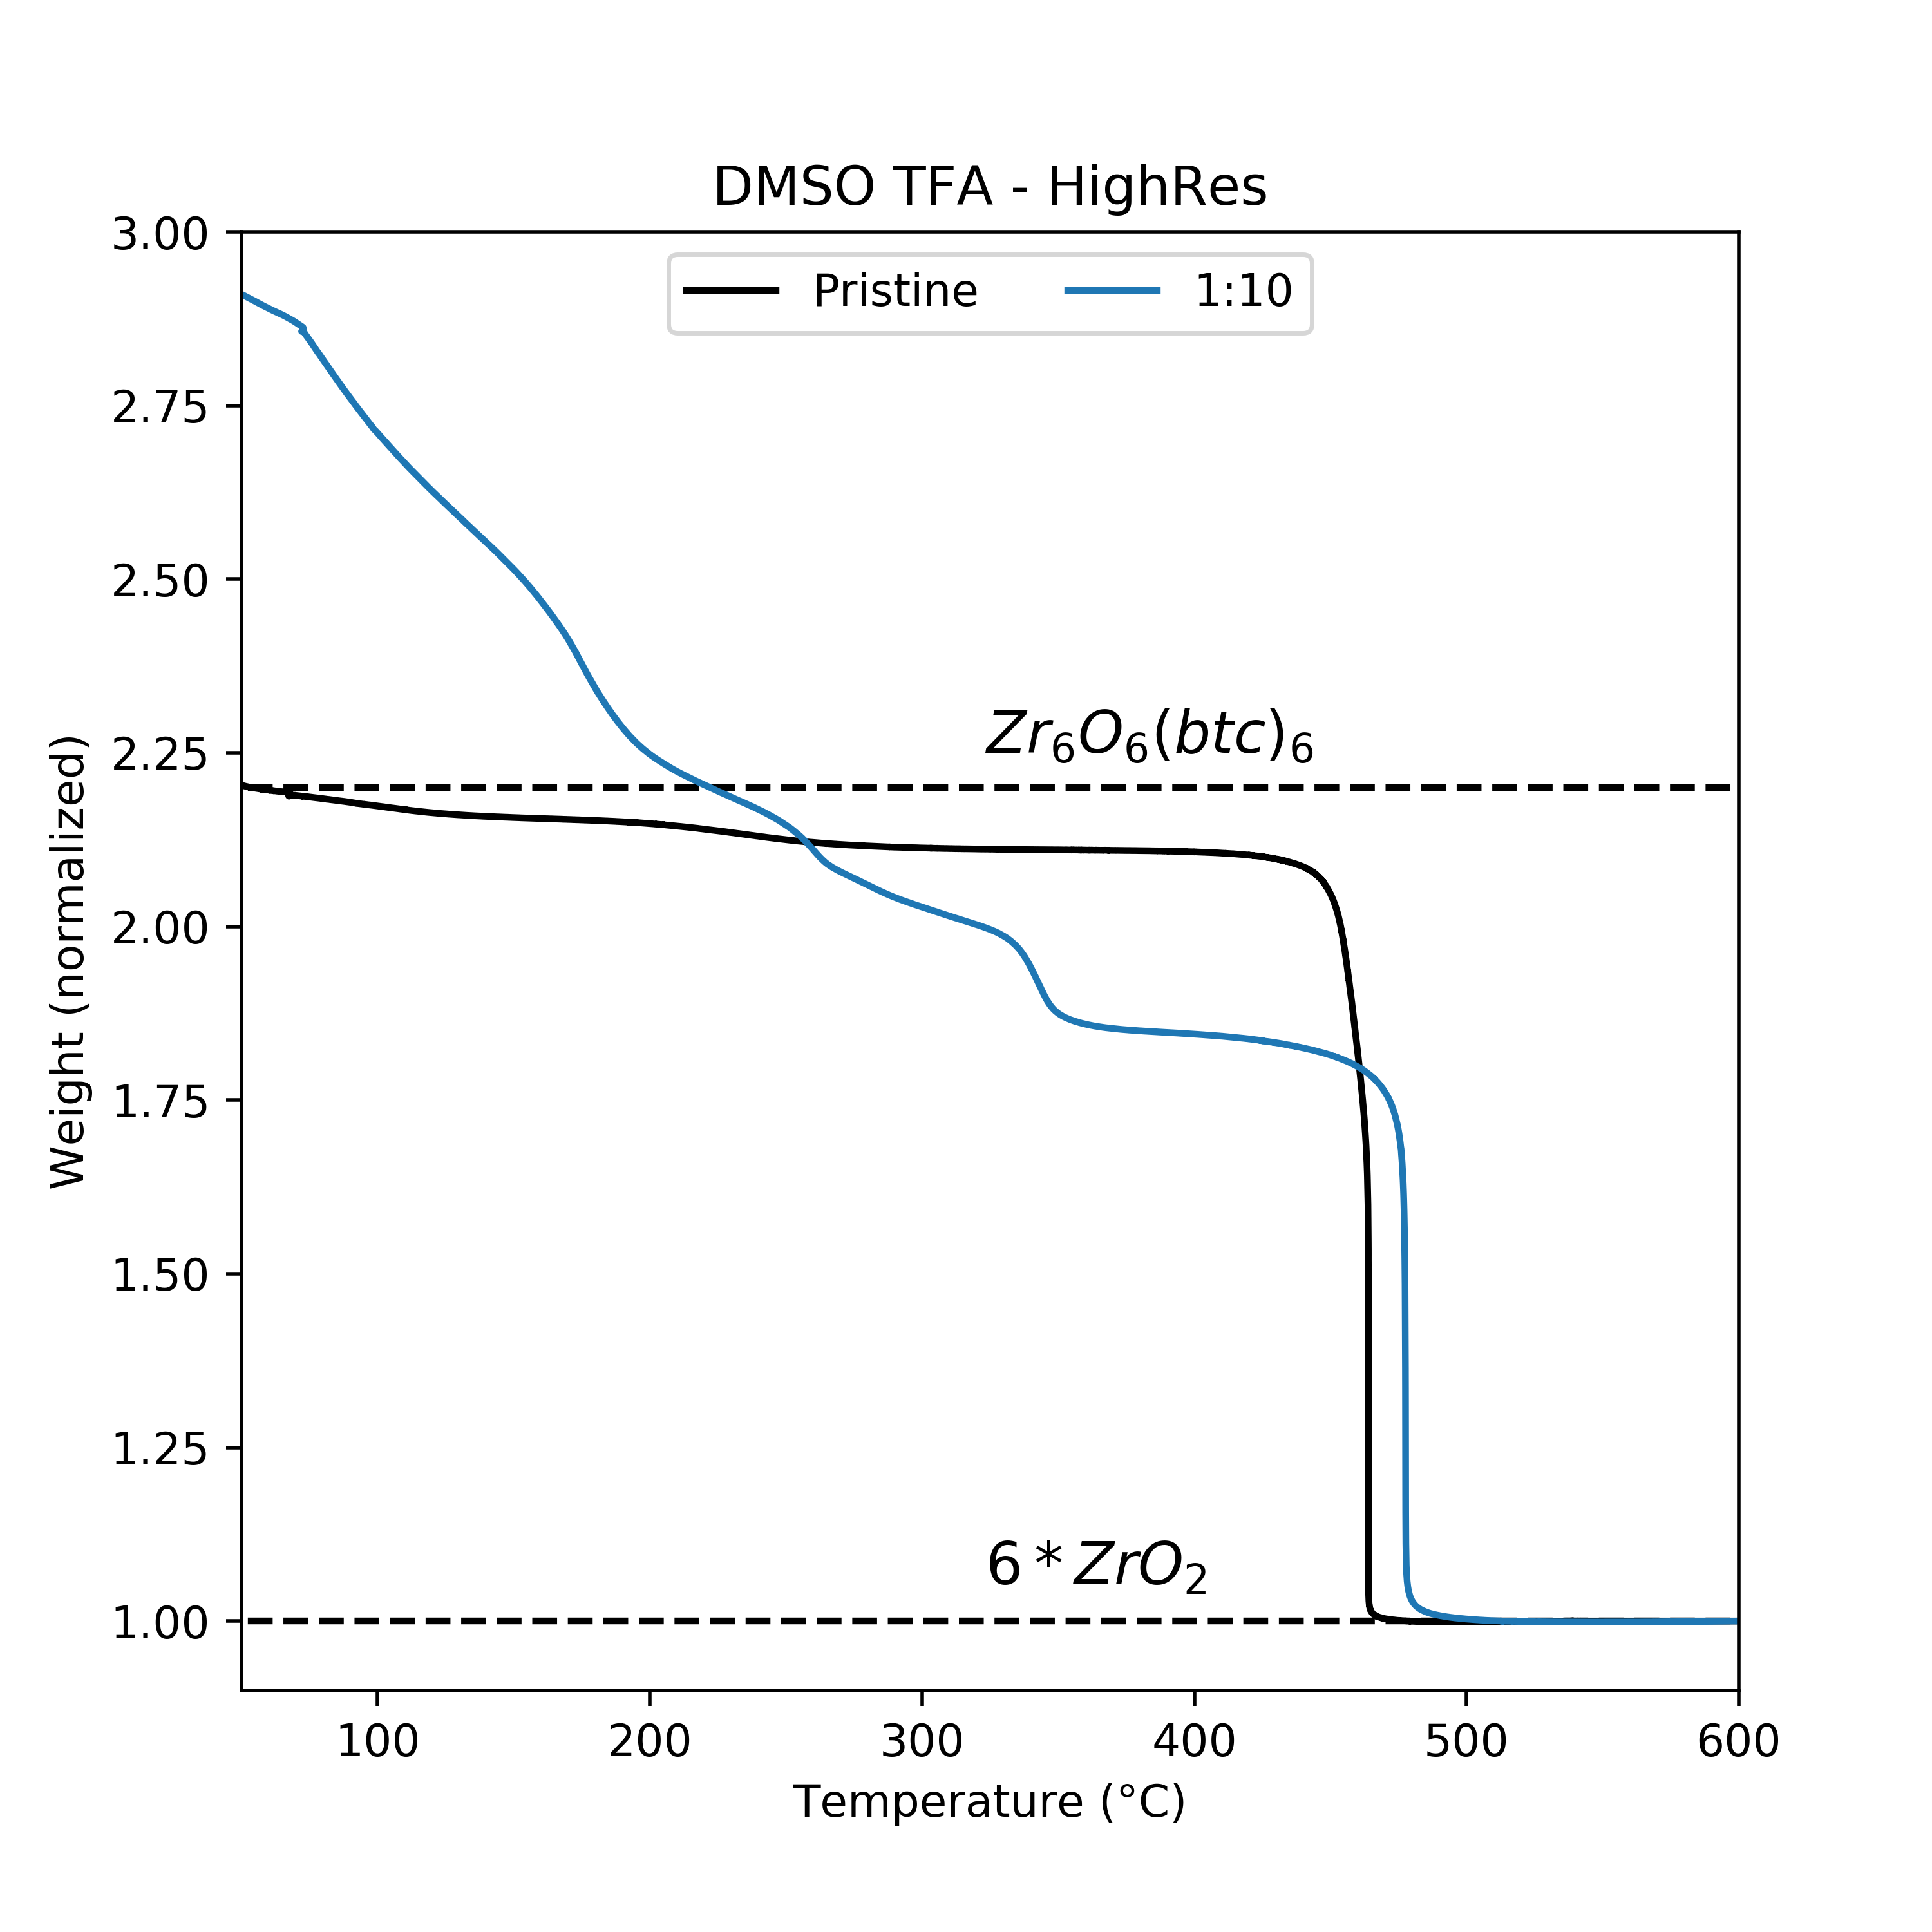
\includegraphics[width=0.5\textwidth]{tga/DMSO-TFA-HR}%
    \caption{High resolution TGA curves for a DMSO/TFA leached sample}%
    \label{appx:def:fgr:tga-dmso-tfa-hr}
\end{figure}

\pagebreak